\documentclass[11pt,a4paper]{article}

\usepackage[margin=2.3cm]{geometry}
\usepackage[T1]{fontenc}
\usepackage[utf8]{inputenc}
\usepackage{lmodern}
\usepackage{microtype}
\usepackage{graphicx}
\usepackage{booktabs}
\usepackage{tabularx}
\usepackage{float}
\usepackage{caption}
\usepackage{subcaption}
\usepackage{amsmath}
\usepackage{xcolor}
\usepackage{enumitem}
\usepackage{url}
\usepackage[hidelinks]{hyperref}

\graphicspath{{figures/}}
\setlist{itemsep=2pt, topsep=4pt}
\setlength{\emergencystretch}{3em}  % long \texttt names cannot hyphenate
\captionsetup{font=small, labelfont=bf}
\newcommand{\code}[1]{\texttt{#1}}
\newcommand{\fig}[1]{Figure~\ref{#1}}
\newcommand{\tab}[1]{Table~\ref{#1}}
\newcommand{\nb}[1]{\textit{(notebook \S#1)}}

\title{\textbf{Formula 1 Podium Prediction}\\[4pt]
\large CSEN903 Advanced Computer Lab --- Milestone 1 Report}
\author{Team members\\[4pt]
  \textit{Abdelhamid Sameh (58-1165)} \\ \textit{Mohamed Ayman (58-8189)} \\
  \textit{Noureldeen Amr (58-1632)} \\ \textit{Noureldin Abdelrahman (58-7007)}}
\date{October 2026}

\begin{document}
\maketitle

\begin{center}
\small
Notebook: \code{notebooks/f1\_podium\_prediction.ipynb}\\
Kaggle: \url{https://www.kaggle.com/code/nooredeenamr/notebook03d3448a5a}\\
GitHub: \url{https://github.com/MohamedAyman04/f1-drivers}
\end{center}

\begin{abstract}
\noindent
We predict, for every driver in every Formula~1 race from 1950 to 2024, whether the driver finishes on the podium (\code{positionOrder} $\le 3$), using only what is known after qualifying and before the start.
The 14 raw tables are audited and cleaned on copies (160{,}076 \verb|\N| sentinels, 85 duplicated driver-race pairs, all keys checked), the three data-engineering questions are answered with multi-hop joins, and a leakage-safe modeling table of 24{,}933 entries is built and split by season.
Feature groups are added one at a time on the validation seasons; only the starting grid and the driver's championship standings before the race earn their place.
A logistic regression, a random forest and a shallow neural network all beat a grid-only baseline: test PR-AUC 0.708, 0.720 and 0.706 against 0.647, with no model clearly ahead of the others.
SHAP and LIME show that every model relies mostly on the grid. These explanations describe the models, not what causes podiums.
Section numbers in the form \nb{9.1} point to the matching section of the notebook, where every number in this report is printed.
\end{abstract}

\tableofcontents
\newpage

%==============================================================================
\section{Task and dataset}

\paragraph{Task.} The unit of analysis is one driver entering one race, identified by \code{(raceId, driverId)}. The target is \code{podium = 1} if \code{positionOrder} $\le 3$, otherwise 0.
The prediction is made \textbf{after qualifying and before the start}. Anything known only during or after the race (finishing position, points, laps, race time, fastest lap, retirement status, standings after the race) would be \emph{leakage} and is never an input.

\paragraph{Dataset.} The Kaggle/Ergast \textit{Formula 1 World Championship (1950--2024)} dataset~\cite{f1dataset}: 14 relational CSV tables. \code{results} (26{,}759 rows) is the central table; its ID columns point to \code{races}, \code{drivers}, \code{constructors} (teams) and \code{status}, and \code{races} points to \code{circuits}. The raw files are never modified: every cleaning step works on copies in memory.

\paragraph{Tools.} pandas, numpy, matplotlib, seaborn and missingno for data handling and plots; scikit-learn~\cite{sklearn} for the statistical models; TensorFlow/Keras for the neural network; shap and lime for the explanations. The notebook runs top to bottom with one \textit{Run All} on Kaggle (CPU only).

%==============================================================================
\section{Exploratory data analysis before cleaning}

\subsection{First look and sentinels}
\code{head}, \code{info} and \code{describe} on \code{results} show the main problem at once: \code{position}, \code{milliseconds}, \code{fastestLap}, \code{rank} and \code{fastestLapSpeed} hold numbers but were read as text, and \code{isnull()} reports no missing values. The dataset writes ``no value'' as the string \verb|\N| (a \emph{sentinel}), which hides missing values from pandas. Over all tables there are 160{,}076 sentinel cells in 30 columns, and \code{isnull()} finds only 68 of them \nb{4}.

\begin{table}[H]
\centering\small
\caption{Columns with the most \texttt{\textbackslash N} sentinels.}
\label{tab:sentinels}
\begin{tabular}{llrr}
\toprule
Table & Column & Sentinels & Share of rows \\
\midrule
results & time, milliseconds & 19{,}079 & 71.3\% \\
results & fastestLap, fastestLapTime, fastestLapSpeed & 18{,}507 & 69.2\% \\
results & rank & 18{,}249 & 68.2\% \\
constructor\_results & status & 12{,}608 & 99.9\% \\
results & position & 10{,}953 & 40.9\% \\
qualifying & q3 / q2 & 6{,}819 / 4{,}625 & 65.0\% / 44.1\% \\
races & sprint\_date & 1{,}107 & 98.4\% \\
\bottomrule
\end{tabular}
\end{table}

\subsection{Where and when values are missing}
\fig{fig:msno-before} shows the missing values of \code{results} and \code{qualifying}, and \fig{fig:coverage} shows how coverage changes over the 75 seasons. The first season with any value is 1994 for Q1 times, 2005 for Q2, 2006 for Q3 and 2004 for fastest-lap times.

\begin{figure}[H]
\centering
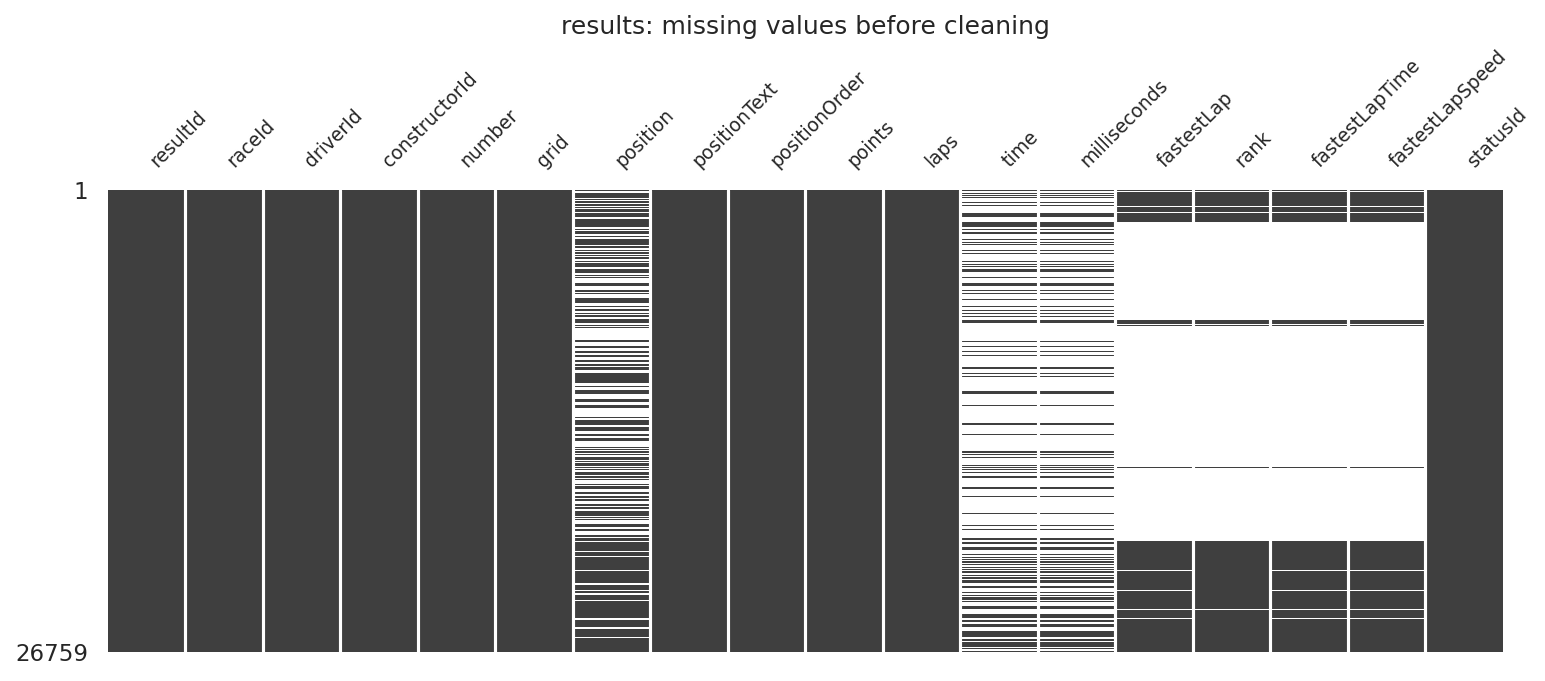
\includegraphics[width=0.49\linewidth]{fig_01_msno_before_results.png}\hfill
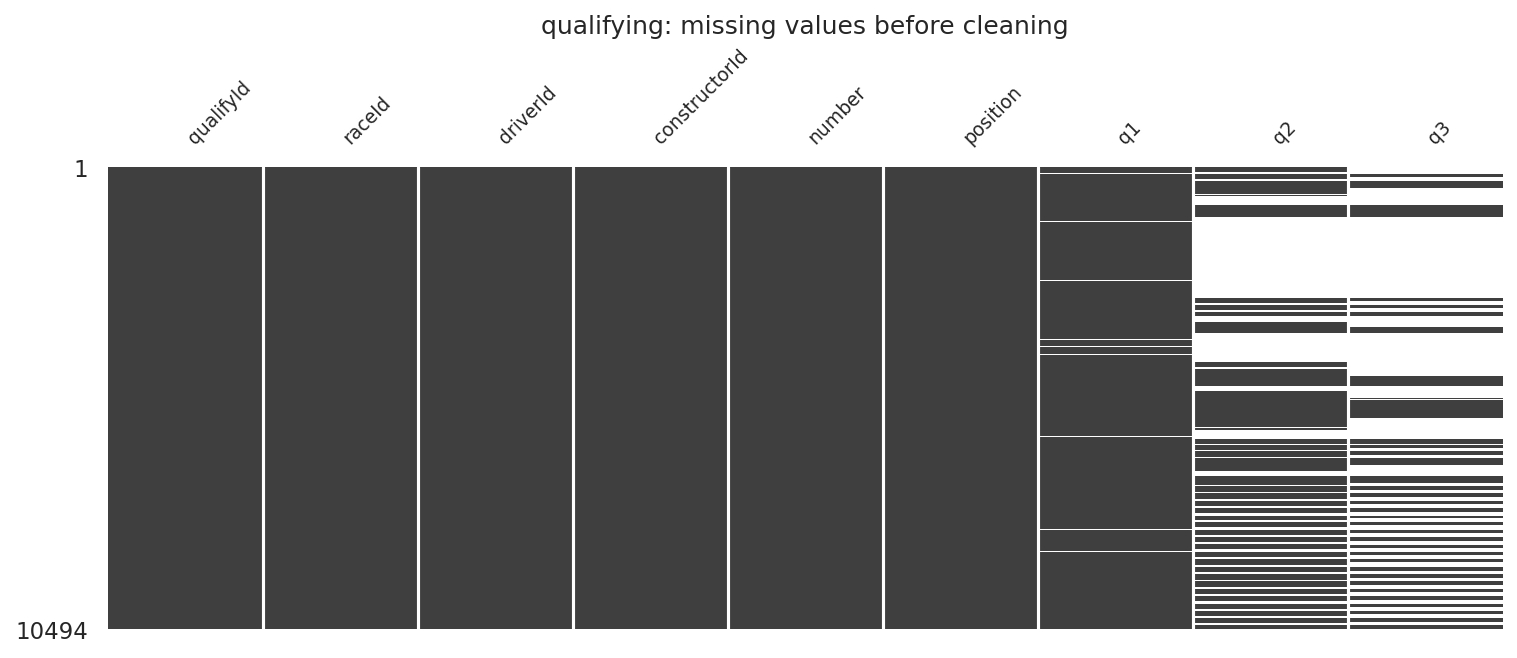
\includegraphics[width=0.49\linewidth]{fig_01_msno_before_qualifying.png}
\caption{Missing values before cleaning (white = missing). In \code{results} they sit in the columns that describe how a race ended.}
\label{fig:msno-before}
\end{figure}

\begin{figure}[H]
\centering
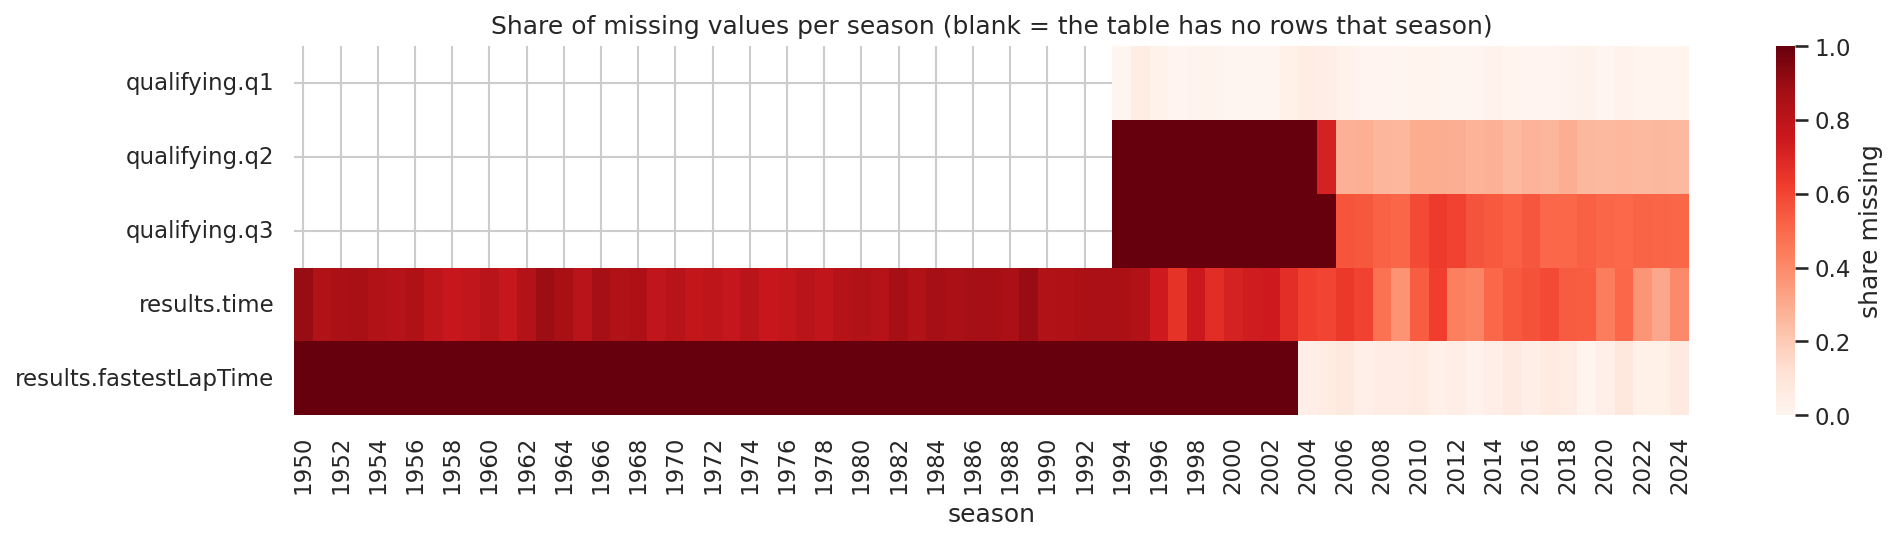
\includegraphics[width=\linewidth]{fig_02_missing_by_season.png}
\caption{Share of missing values per season (blank = no rows that season). Even after 2006, Q2/Q3 are partly empty because only the faster drivers reach them (28\%/55\% missing in 2014, 25\%/51\% in 2024).}
\label{fig:coverage}
\end{figure}

\subsection{Spelling, grid slots and field sizes}
Every name-like text column was checked with the same rules: spaces at the start or end, HTML codes, and values that become identical once case, accents and punctuation are ignored. Nationalities and circuit countries (compared in Q2) got extra checks for compound values, abbreviations and shared first letters. Found: \code{'Argentinian '} (with a trailing space) next to \code{Argentine}; \code{United States} next to \code{USA}; two compound nationalities (\code{American-Italian}, \code{Argentine-Italian}); \code{East German}; and one HTML code (\code{Lotus-Pratt \&amp; Whitney}). Four first names differ only by an accent (\code{Adrian}/\code{Adri\'an}), but they belong to different drivers and no analysis uses first names, so they are left alone \nb{4.1}.

\begin{figure}[H]
\centering
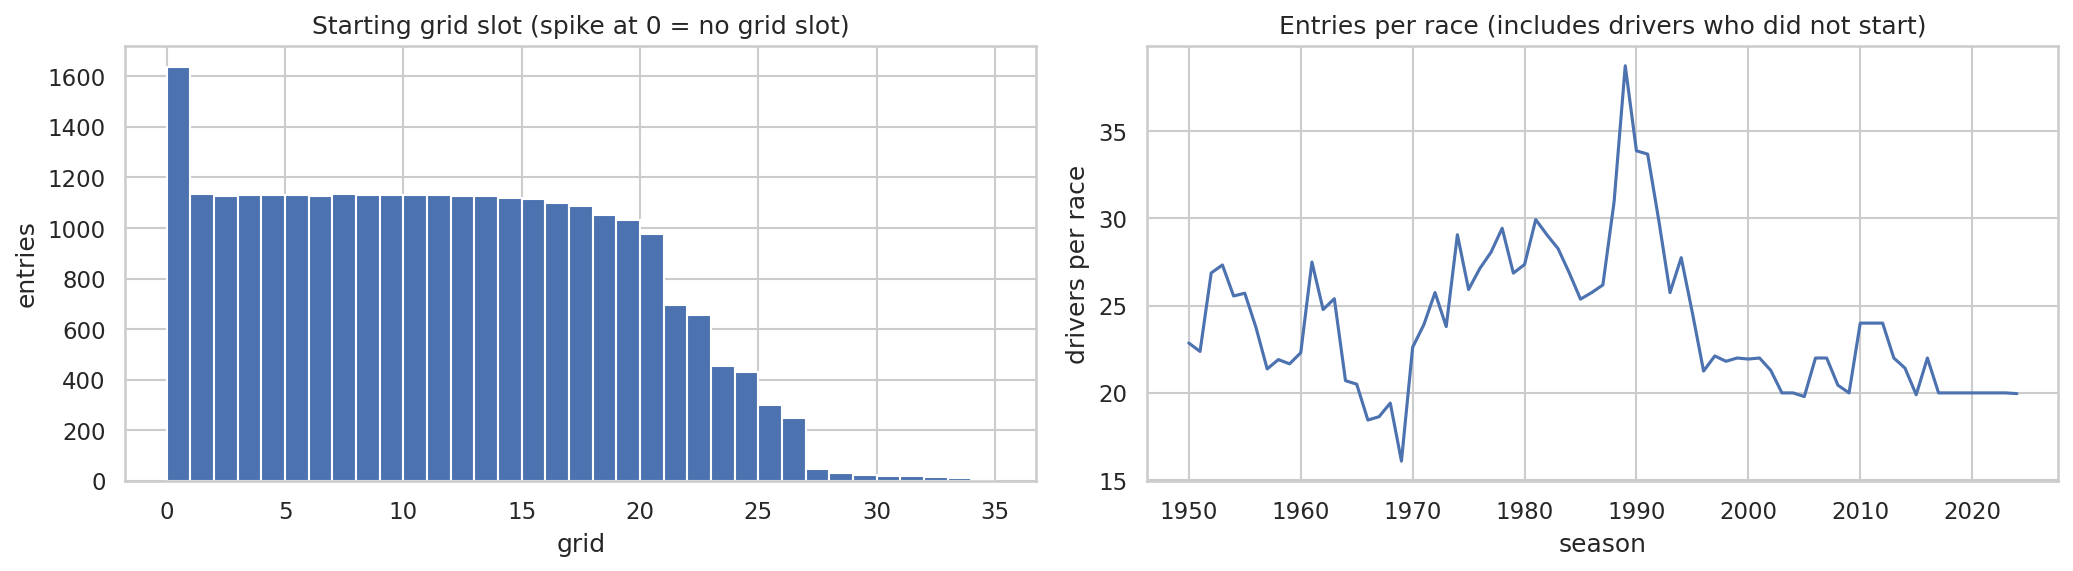
\includegraphics[width=\linewidth]{fig_03_grid_and_entries.png}
\caption{Left: starting grid slot, with a spike at 0. Right: entries per race, including drivers who never started.}
\label{fig:grid}
\end{figure}

\code{grid = 0} occurs 1{,}638 times and means two things: 72 pit-lane starters (who drove laps) and entries that never started (\fig{fig:grid}). Until the 1990s many more drivers entered a race than could start.

\subsection{Keys and duplicates}
\begin{itemize}
\item \textbf{Primary keys} are found by rule, not typed in: the first column if it is an ID and unique; for \code{lap\_times} and \code{pit\_stops} the lap or stop counter is added to \code{(raceId, driverId)}. All 14 keys are unique and never empty.
\item \textbf{Foreign keys} are every column named like another table's key. All 23 links have 0 orphans. The notebook stops if either check fails \nb{5}.
\item \textbf{Duplicates.} 85 \code{(raceId, driverId)} pairs appear more than once (176 rows), all between 1950 and 1978. In all 85 pairs the rows have different car numbers: these are \emph{shared drives}, where a driver drove more than one car in the same race \nb{5.1}.
\end{itemize}

\paragraph{Duplicate rule.} We keep the row with the \textbf{lowest real grid slot}, taken as the car the driver started in; ties (1 pair) and pairs without a slot (3 pairs) are decided by the better finish. The rule matters for the label: keeping the best finish would give 22 podiums instead of 5, because a driver who took over a teammate's car would be credited with that car's result. Our rule keeps the car that the pre-race input (\code{grid}) describes. All 85 pairs are in training seasons.

%==============================================================================
\section{Cleaning}

All cleaning works on copies. Missing values are \emph{not} filled here; filling happens later with training statistics only (Section~\ref{sec:prep}).

\begin{table}[H]
\centering\small
\caption{Cleaning steps and their effect \nb{6}.}
\label{tab:cleaning}
\begin{tabularx}{\linewidth}{lX}
\toprule
Step & What it does and its effect \\
\midrule
1. Sentinels & \verb|\N| $\rightarrow$ NaN (160{,}076 cells); spaces trimmed; HTML codes decoded; text columns whose values are all numbers become numbers (6 in \code{results}, 1 in \code{drivers}, 3 in \code{sprint\_results}). \\
2. Semantic typing & Dates $\rightarrow$ \code{datetime}; lap times and durations (\code{"1:27.452"}) $\rightarrow$ seconds. The parsed lap and pit-stop times match the dataset's own millisecond columns exactly (asserted). \\
3. One spelling per value & The more common spelling is kept (\code{United States} $\rightarrow$ \code{USA}, \code{Argentinian} $\rightarrow$ \code{Argentine}); compound nationalities keep the first; \code{East German} $\rightarrow$ \code{German}. Every driver gets a \code{home\_country} in the circuits' spelling (asserted complete); 14 home countries never hosted a race. \\
4. Unused columns & Web links and practice/qualifying/sprint session dates dropped. \\
5. One row per driver-race & The duplicate rule above: 26{,}759 $\rightarrow$ 26{,}668 rows; uniqueness asserted. \\
6. Flags & 1{,}354 entries whose status is ``Did not qualify'' or ``Did not prequalify'' are removed from modeling and Q3 (12 of them still carry a grid number, a data error). 221 entries qualified but did not start: kept, as honest ``no'' rows (0 podiums). 72 pit-lane starters kept. Entries without a slot get the slot behind the last car (\code{grid\_eff}). 381 Indianapolis~500 rows (1950--1960) flagged and excluded. \\
7. Status classes & 137 statuses grouped by reading them: finished (15{,}115 rows), mechanical (6{,}775), accident (2{,}771), regulatory (1{,}942), driver (65). Nine statuses that do not say what failed (\code{Retired}, \code{Puncture}, \code{Out of fuel}, \dots) count as mechanical and are flagged as unclear. Used in Q3. \\
\bottomrule
\end{tabularx}
\end{table}

\paragraph{Evidence for the rules \nb{6.1}.} Pit-lane starters finish like the last three grid slots (median finishing position 15 for both; 0 podiums in 72 pit-lane starts), so ``one slot behind the last car'' fits. Of 381 Indy~500 driver-seasons, only 2 (1\%) also raced another championship race that season, so it was a separate race with its own drivers.

\paragraph{Effect of the cleaning.} The former sentinel columns are numbers, and missing values are visible to pandas. Removing the entries that did not qualify brings the number of drivers per race down to the real fields (\fig{fig:after}).

\begin{figure}[H]
\centering
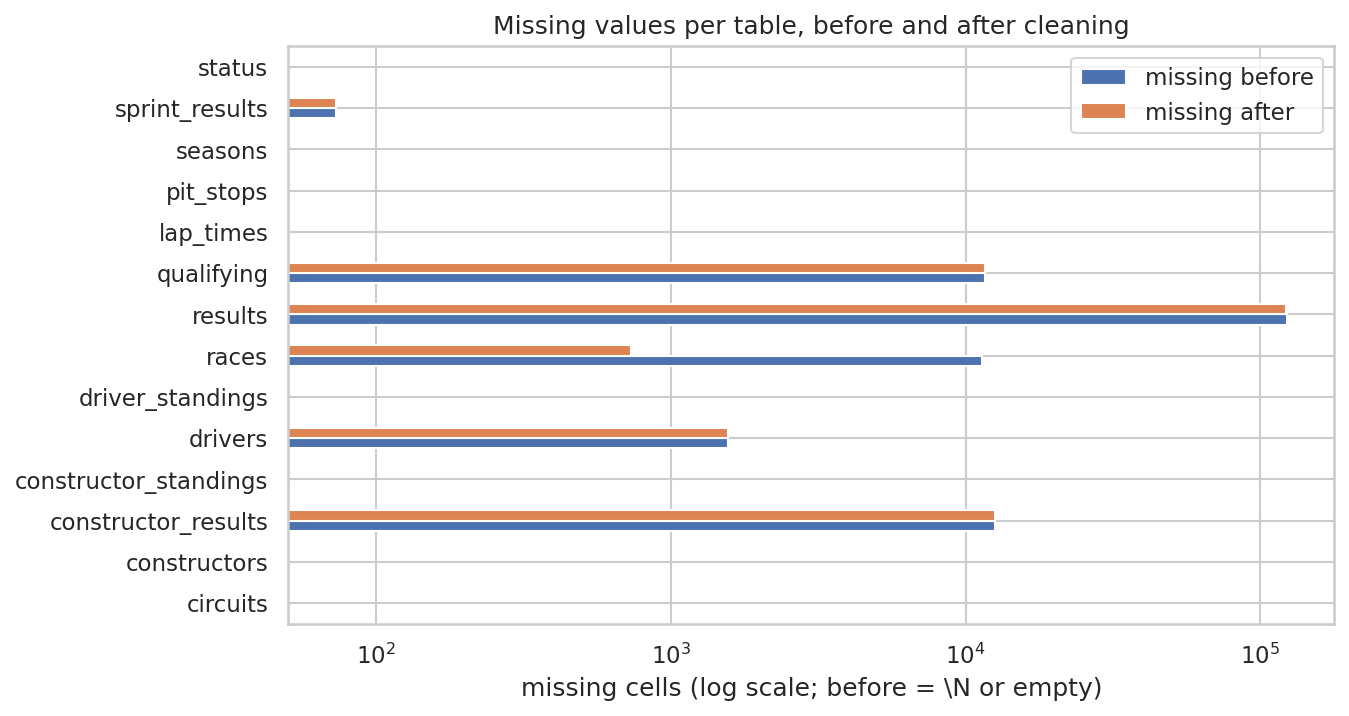
\includegraphics[width=0.62\linewidth]{fig_04_missing_before_after.png}\\[4pt]
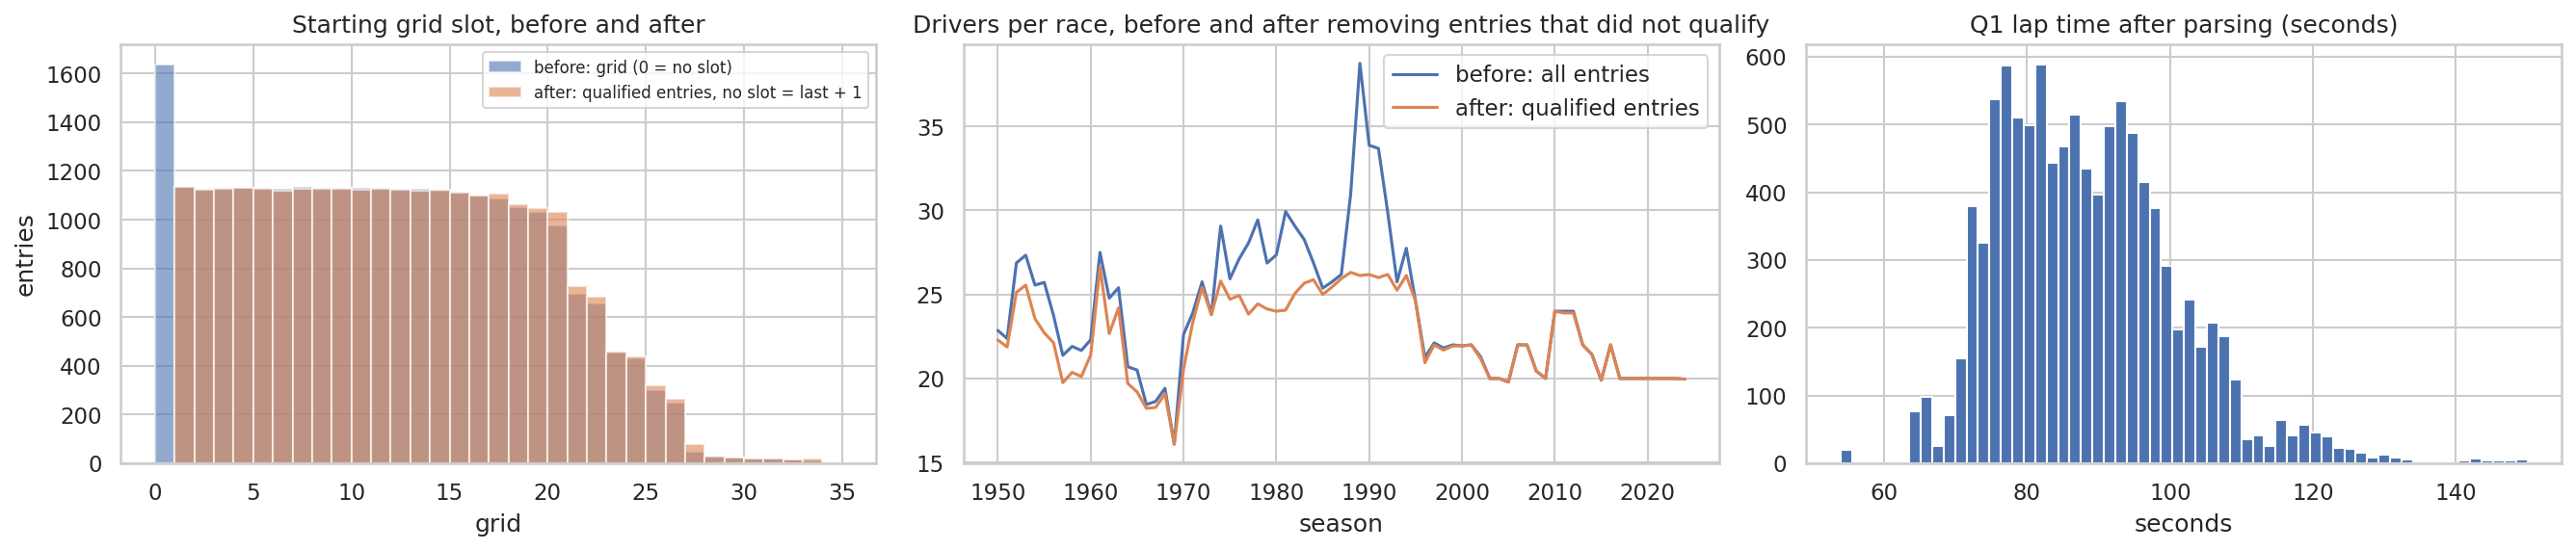
\includegraphics[width=\linewidth]{fig_05_after_cleaning.png}
\caption{After cleaning. Top: missing cells per table before and after (log scale). Bottom: grid slots, drivers per race before and after removing non-qualifiers, and Q1 lap times after parsing to seconds.}
\label{fig:after}
\end{figure}

%==============================================================================
\section{Target, pre-race cutoff and metrics}

Every driver who qualified is counted, including the few who did not start: 13.3\% of entries end on the podium (3{,}378 of 25{,}314), so the classes are imbalanced. The rate follows $3/\text{starters per race}$ (\fig{fig:target}), so it is about 10\% in the large fields of the 1950s--80s and about 15\% today. This era shift is one reason the data is split by season.

\begin{figure}[H]
\centering
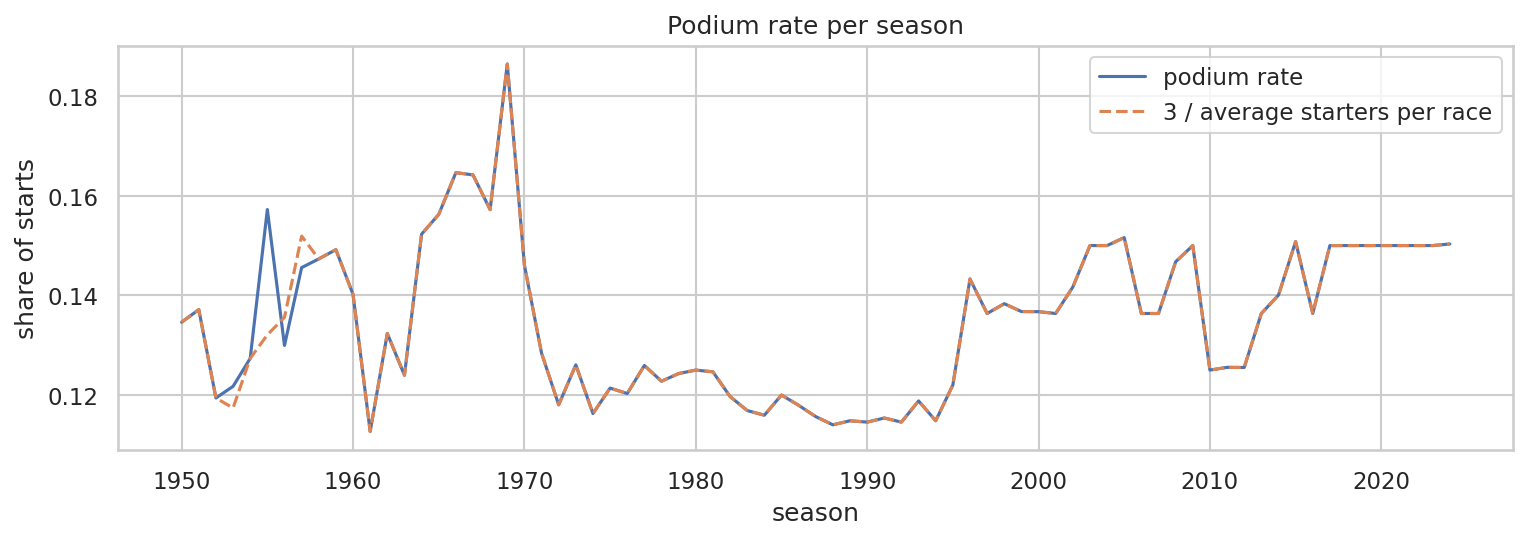
\includegraphics[width=0.9\linewidth]{fig_06_podium_rate.png}
\caption{Podium rate per season and $3/\text{average starters per race}$. The lines part only in a few 1950s races with shared drives.}
\label{fig:target}
\end{figure}

\begin{table}[H]
\centering\small
\caption{The pre-race cutoff.}
\label{tab:cutoff}
\begin{tabularx}{\linewidth}{XX}
\toprule
Allowed (known before the start) & Not allowed (only known after the race) \\
\midrule
\code{grid} (qualifying result after penalties) & \code{position}, \code{positionText}, \code{positionOrder}, \code{points} \\
driver, team and circuit identity & \code{laps}, \code{time}, \code{milliseconds}, \code{statusId} \\
championship standings \textbf{after the previous round} & \code{fastestLap}, \code{rank}, \code{fastestLapTime}, \code{fastestLapSpeed} \\
results of \textbf{earlier} races & this race's \code{lap\_times}, \code{pit\_stops}, and standings after this race \\
\bottomrule
\end{tabularx}
\end{table}

\paragraph{Sprints.} A sprint result is known before Sunday's race, so it would be allowed. But only 18 of 1{,}125 races have a sprint, and sprints only started in 2021 (general knowledge), so none falls in the training seasons and the feature would be empty for every training row. Sprint results are not used.

\paragraph{Metric choice.} A model that always says ``no podium'' is about 87\% accurate and useless, so accuracy is only reported for reference.
The \textbf{primary metric is PR-AUC} (average precision): how well the real podium finishers are ranked above everyone else, focused on the rare class.
The \textbf{secondary metrics} are ROC-AUC (overall separation of the classes) and F1 at a threshold chosen on validation (the quality of the actual yes/no decision). Precision, recall and accuracy are reported next to F1.

%==============================================================================
\section{Data-engineering questions}

Each answer joins several tables, and after every join the notebook asserts that the number of rows did not change. The answers describe the data and are not used to choose anything in the modeling, so they may look at all seasons.
Rates come with 95\% Wilson intervals~\cite{wilson1927,agresti1998}: the simple ``rate $\pm$ 1.96 standard errors'' breaks for small counts (0 of 12 gives $0\% \pm 0$; 1 of 12 gives a lower end of $-7.3\%$), while Wilson's interval stays inside 0--100\% and widens when there are few cases. If two intervals do not overlap, the difference is very unlikely to be chance.

\subsection{Q1: Which circuits convert a front-row start into a podium most often, and did that change after 2014?}

\paragraph{Method.} \code{results} $\rightarrow$ \code{races} $\rightarrow$ \code{circuits}. \textbf{Grain:} one front-row start (grid slot 1 or 2), 2{,}259 rows, unique per \code{(raceId, driverId)}. \textbf{Qualifying vs.\ grid:} they can differ because of penalties; we use \code{grid}, the slot the car actually started from, which exists for every race since 1950 (qualifying positions start in 1994). \textbf{Missingness:} \code{grid} and \code{positionOrder} are never missing. \textbf{Cutoff:} the starting slot is known before the start; the podium is the outcome being counted.
A circuit is ranked only with at least 10 front-row starts (about 5 races) in \emph{each} era: a circuit used once has 2 front-row starts, so its rate can only be 0\%, 50\% or 100\%. Of 77 circuits, 45 were raced only before 2014 and 8 only from 2014; of the 24 raced in both eras, 16 pass the minimum.

\begin{figure}[H]
\centering
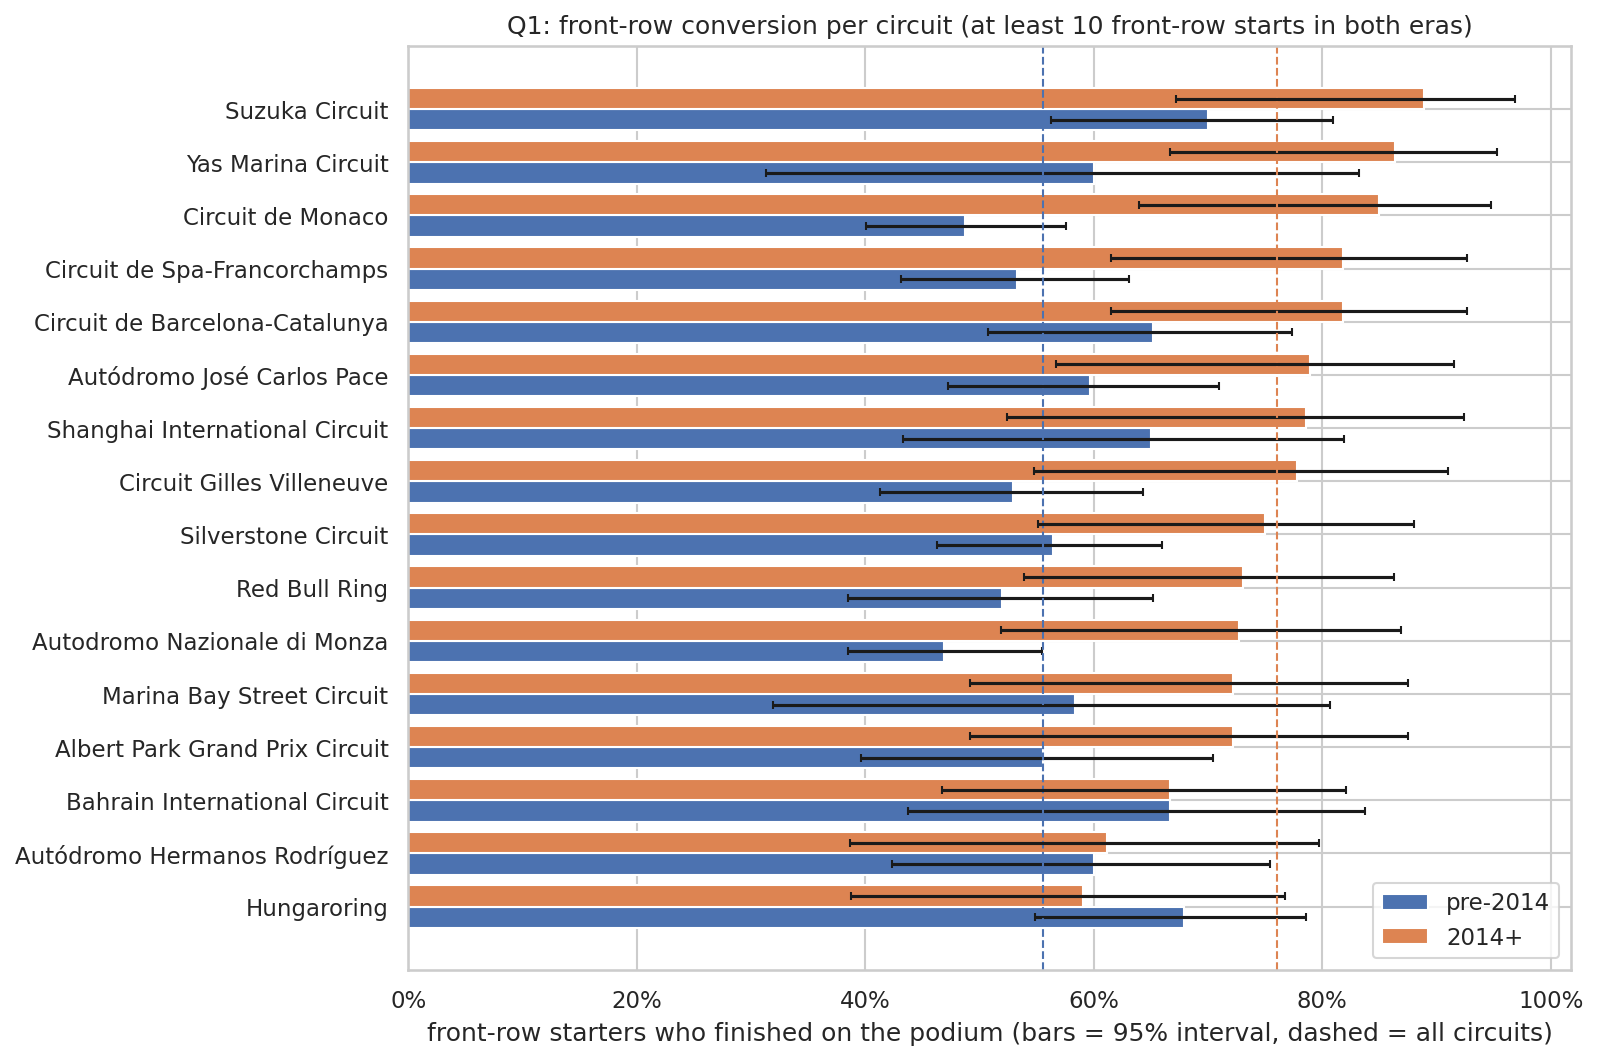
\includegraphics[width=0.6\linewidth]{fig_07_q1_circuits.png}\hfill
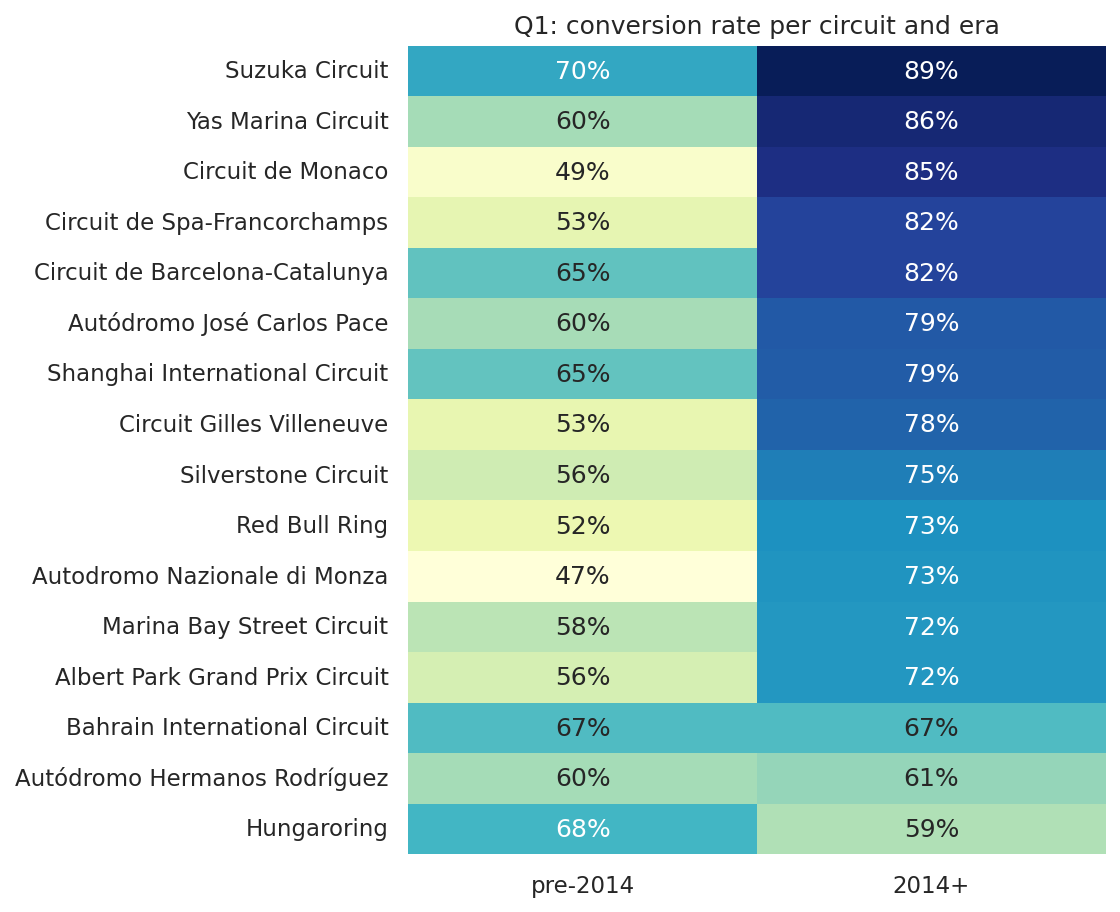
\includegraphics[width=0.39\linewidth]{fig_08_q1_heatmap.png}
\caption{Q1: front-row conversion per circuit, before 2014 and from 2014 (bars = 95\% intervals, dashed = all circuits), and the same rates as a heatmap.}
\label{fig:q1}
\end{figure}

\paragraph{Answer.} A front-row start converts much more often in the hybrid era: \textbf{55.5\% before 2014} (1{,}002 of 1{,}805; 53.2--57.8\%) \textbf{vs.\ 76.0\% from 2014} (345 of 454; 71.9--79.7\%); the intervals do not overlap.
The best circuits since 2014 are Suzuka (16 of 18, 89\%), Yas Marina (86\%) and Monaco (85\%).
The ranking is \textbf{not stable}: the Spearman rank correlation between the eras is $-0.03$ ($p = 0.91$, 16 circuits). Monaco went from 15th of 16 (49\%) to 3rd, and the Hungaroring from 2nd (68\%) to last (59\%). With other minimums (6, 14 or 20 starts) the correlation stays between $-0.18$ and $0.06$, and Suzuka stays on top for 6 and 14.

\subsection{Q2: Do drivers podium more often at home, for the same starting position?}

\paragraph{Method.} \code{results} $\rightarrow$ \code{drivers} $\rightarrow$ \code{races} $\rightarrow$ \code{circuits}. A home race is a race in the driver's \code{home\_country} (cleaning step~3). \textbf{Grain:} one qualified entry, without the Indy~500: 24{,}933 starts, 1{,}974 at home (7.9\%). \textbf{Missingness:} every driver has a home country and every circuit a country. \textbf{Cutoff:} home status and starting position are known before the start.
Home drivers might simply qualify better, so the rates are compared \emph{within} starting groups (pole, 2--3, 4--6, 7--10, 11+), and the home-minus-away gaps are averaged, weighted by home starts. A logistic regression of podium on home, starting group and era (dummy columns, one category left out as reference, effectively no regularisation) gives the home effect as an \textbf{odds ratio}: 1 = no effect, below 1 = home does worse.

\begin{table}[H]
\centering\small
\caption{Q2: podium rate by starting group, home vs.\ away.}
\label{tab:q2}
\begin{tabular}{lrrrrr}
\toprule
Start & Away rate & Home rate & Home -- away & Home starts & Away starts \\
\midrule
Pole & 64.2\% & 58.3\% & $-5.9$ pp & 84 & 1{,}040 \\
2--3 & 50.9\% & 53.7\% & $+2.9$ pp & 147 & 2{,}078 \\
4--6 & 26.0\% & 26.4\% & $+0.4$ pp & 227 & 3{,}114 \\
7--10 & 9.2\% & 7.1\% & $-2.1$ pp & 336 & 4{,}117 \\
11+ & 1.6\% & 1.0\% & $-0.6$ pp & 1{,}180 & 12{,}610 \\
\bottomrule
\end{tabular}
\end{table}

\begin{figure}[H]
\centering
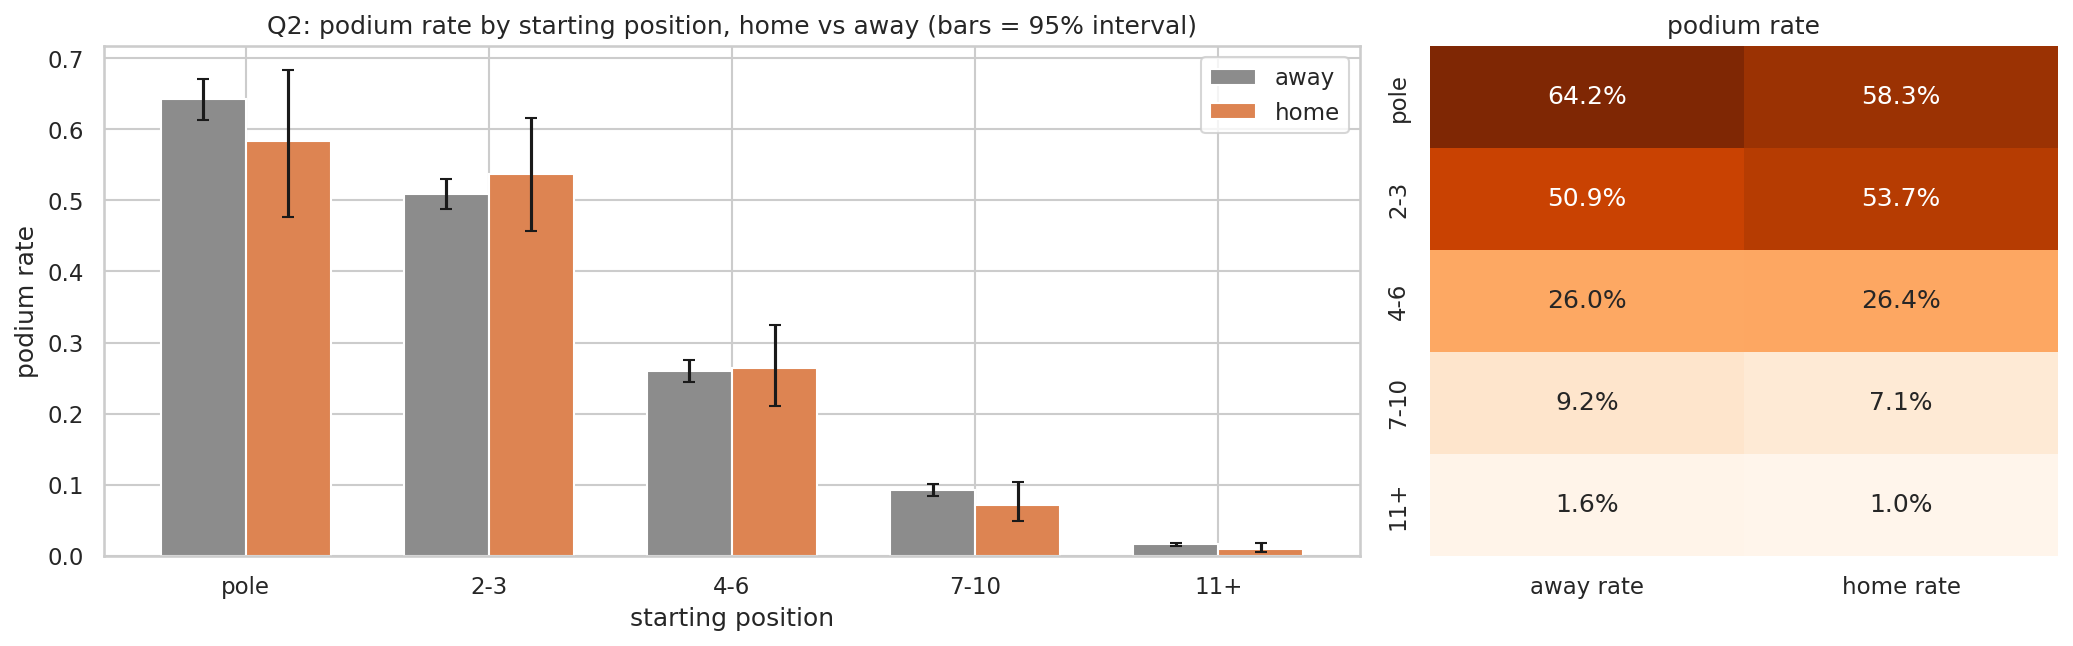
\includegraphics[width=\linewidth]{fig_09_q2_home.png}
\caption{Q2: podium rate by starting position, home vs.\ away (bars = 95\% intervals).}
\label{fig:q2}
\end{figure}

\paragraph{Answer.} \textbf{No home advantage.} From the same starting group, home drivers are 0.70 percentage points \emph{less} likely to finish on the podium, and the odds ratio is \textbf{0.912}. In every starting group the home and away intervals overlap, so the small negative gap cannot be told apart from no effect. The odds ratio stays between 0.894 and 0.912 with other era splits (none, 2014 only, decades).

\subsection{Q3: Which constructors have the highest mechanical-retirement rate in 2014--2021 vs.\ 2022--2024?}

\paragraph{Method.} \code{results} $\rightarrow$ \code{status} (class from cleaning step~7) $\rightarrow$ \code{constructors}. \textbf{Grain:} one race start in 2014--2024 (4{,}619 rows); entries that never started are left out, because the brief defines a mechanical retirement as a race start that ended early. \textbf{Definition:} a part of the car failed; crashes, driver causes and rule decisions are excluded. \textbf{Missingness:} every entry has a status and so a class. \textbf{Cutoff:} Q3 describes how races ended, so it uses post-race data on purpose; none of it is a model input.
A team is \emph{clearly less reliable} than its period if even the low end of its interval is above the period's average. The periods differ in length, so rates are compared, never counts. Teams are compared under the name in the data; renames (Toro Rosso $\rightarrow$ AlphaTauri $\rightarrow$ RB, Sauber $\rightarrow$ Alfa Romeo $\rightarrow$ Sauber, \dots) are general knowledge from the teams' Wikipedia pages, and the seasons per name in the data fit them.

\begin{figure}[H]
\centering
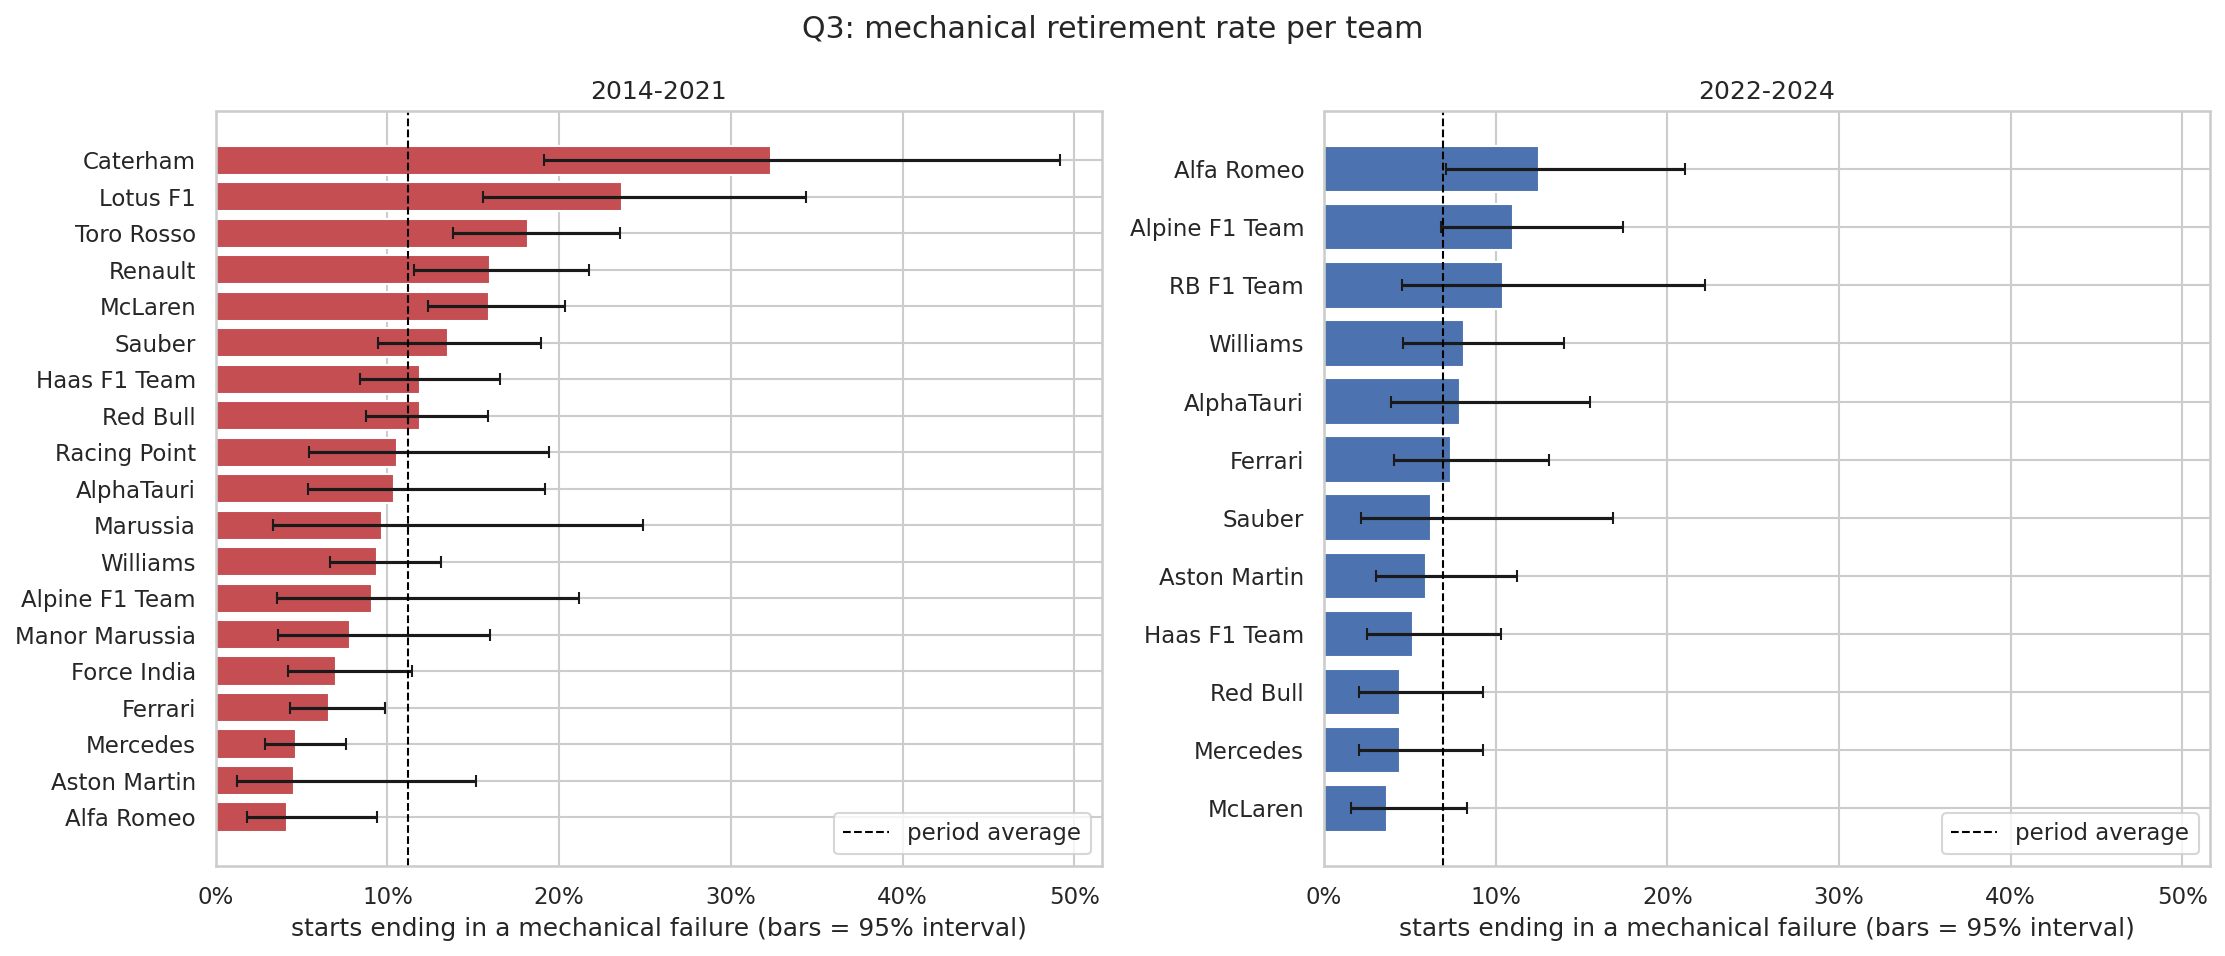
\includegraphics[width=\linewidth]{fig_10_q3_teams.png}
\caption{Q3: mechanical retirement rate per team and period (bars = 95\% intervals, dashed = period average).}
\label{fig:q3}
\end{figure}

\begin{table}[H]
\centering\small
\caption{Q3: highest mechanical-retirement rates per period.}
\label{tab:q3}
\begin{tabular}{llrrr}
\toprule
Period & Team & Starts & Mechanical & Rate \\
\midrule
2014--2021 & Caterham & 34 & 11 & 32.4\% \\
2014--2021 & Lotus F1 & 76 & 18 & 23.7\% \\
2014--2021 & Toro Rosso & 242 & 44 & 18.2\% \\
\midrule
2022--2024 & Alfa Romeo & 88 & 11 & 12.5\% \\
2022--2024 & Alpine F1 Team & 136 & 15 & 11.0\% \\
2022--2024 & RB F1 Team & 48 & 5 & 10.4\% \\
\bottomrule
\end{tabular}
\end{table}

\begin{figure}[H]
\centering
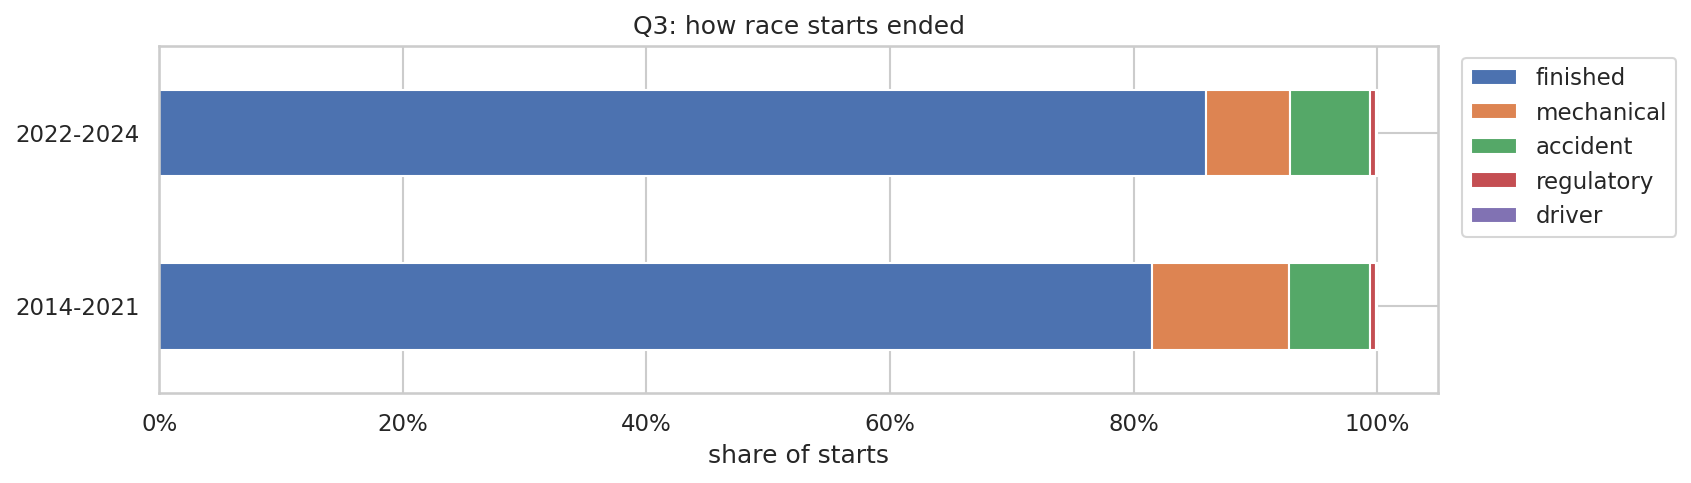
\includegraphics[width=0.85\linewidth]{fig_11_q3_outcomes.png}
\caption{Q3: how race starts ended in each period.}
\label{fig:q3b}
\end{figure}

\paragraph{Answer.} Cars became more reliable: \textbf{11.2\%} of starts in 2014--2021 (366 of 3{,}263; 10.2--12.3\%) vs.\ \textbf{6.9\%} in 2022--2024 (94 of 1{,}356; 5.7--8.4\%) ended with a mechanical failure; the intervals do not overlap. The highest rates were Caterham, Lotus F1 and Toro Rosso in 2014--2021, and Alfa Romeo, Alpine and RB in 2022--2024 (\tab{tab:q3}). Caterham's 32\% rests on 34 starts (interval 19--49\%). Clearly less reliable than their period: Caterham, Lotus F1, McLaren, Renault and Toro Rosso in 2014--2021, and only Alfa Romeo in 2022--2024.
Without the unclear statuses the rates fall to 9.7\% and 6.0\% and the top 3 stays the same, except that AlphaTauri takes RB's third place in 2022--2024.

%==============================================================================
\section{Modeling table and data split}\label{sec:split}

One row per driver who \emph{qualified} for a race in 1950--2024 (including the few who did not start), without the Indy~500: \textbf{24{,}933 rows}, \code{(raceId, driverId)} unique (asserted). Entries without a grid slot start one slot behind the last car.

\begin{table}[H]
\centering\small
\caption{Season-based split \nb{9}.}
\label{tab:split}
\begin{tabular}{llrrrl}
\toprule
Part & Seasons & Rows & Podiums & Rate & Used for \\
\midrule
Train & 1950--2017 & 21{,}954 & 2{,}895 & 13.2\% & fitting models, imputer, scaler \\
Validation & 2018--2021 & 1{,}620 & 243 & 15.0\% & features, settings, thresholds \\
Test & 2022--2024 & 1{,}359 & 204 & 15.0\% & final scores, used once \\
\bottomrule
\end{tabular}
\end{table}

\paragraph{Why split by season.} The task is to predict future races. A random split would put drivers of the same race on both sides and train on seasons later than the ones scored, which makes scores look better than they are. A season split always scores the model on years it has never seen, and the test block is the newest set of car rules (2022--2024).

%==============================================================================
\section{Feature engineering and selection}

\subsection{Candidate features and why they are valid at the cutoff}

\begin{table}[H]
\centering\small
\caption{Candidate features (11 in 5 groups). All use only information from before the race.}
\label{tab:candidates}
\begin{tabularx}{\linewidth}{llX}
\toprule
Group & Features & Why it is known before the start \\
\midrule
grid & \code{grid} & Set by qualifying and penalties before the start (no slot = behind the last car). \\
field size & \code{field\_size}, \code{grid\_rel} & Cars in the race and grid $\div$ cars; the field is fixed once the grid is. \\
driver standings & \code{drv\_pos}, \code{drv\_pts\_share}, \code{drv\_wins} & Position, points $\div$ leader's points, and wins from the standings \textbf{after the previous round} of the same season. \\
team standings & \code{con\_pos}, \code{con\_pts\_share}, \code{con\_wins} & The same for the team. \\
recent form & \code{drv\_form}, \code{con\_form} & Podium share in the driver's (team's) last \code{FORM\_WINDOW} races \emph{before} this one; for a team, the share of its cars. \\
\bottomrule
\end{tabularx}
\end{table}

There are no qualifying-time features: qualifying times exist only from 1994, and the grid already holds the qualifying result after penalties. Points are a share of the leader's points, because raw points are not comparable across points systems (\fig{fig:engineered}). Driver and team identity enter only through these features; one-hot encoding 861 driver IDs would add hundreds of mostly empty columns, and many test drivers never appear in training.

\begin{figure}[H]
\centering
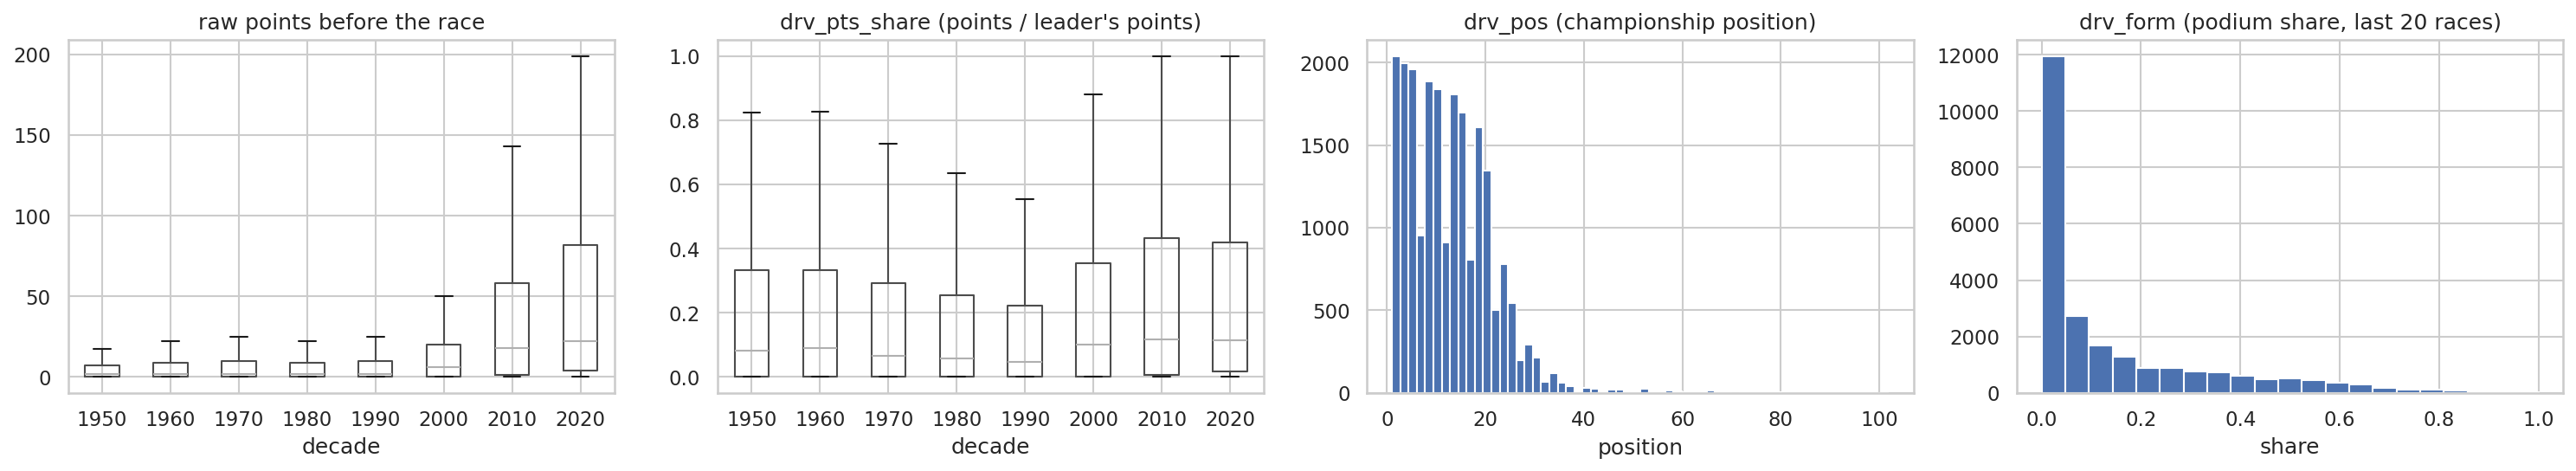
\includegraphics[width=\linewidth]{fig_11c_engineered_features.png}
\caption{Engineered features on all rows: raw points and the points share per decade (the share always runs from 0 to 1), championship positions, and driver form.}
\label{fig:engineered}
\end{figure}

\subsection{How many races should recent form look back?}\label{sec:window}
For windows of 1 to 150 races, the two form features are built and a logistic regression on \code{grid} + both features is scored on validation \nb{9.1}. One validation score is not exact, so the rule is: \textbf{the shortest window that validation cannot tell apart from the best one}, because a shorter window reacts faster when the order of the teams changes. Whether two windows can be told apart is checked with a \textbf{race bootstrap}~\cite{efron1993}: the validation races are drawn at random with repeats (whole races, because the drivers of one race share one result), both windows are rescored on the drawn rows, and this is repeated 2{,}000 times; the middle 95\% of the differences is the 95\% range of the gap. If it reaches 0, validation cannot tell the two windows apart.

\begin{table}[H]
\centering\footnotesize
\caption{Form window: Spearman correlation of each form feature with the podium (train), validation PR-AUC of a logistic regression on grid + both form features, and its gap to the best window with the 95\% bootstrap range \nb{9.1}.}
\label{tab:window}
\begin{tabular}{rrrrrc}
\toprule
Window & Driver form $\rho$ & Team form $\rho$ & Val PR-AUC & Gap to best (95\% range) & As good as best \\
\midrule
1 & 0.330 & 0.360 & 0.681 & $-0.049$ ($-0.084$ to $-0.014$) & no \\
3 & 0.414 & 0.406 & 0.692 & $-0.038$ ($-0.070$ to $-0.005$) & no \\
5 & 0.434 & 0.412 & 0.691 & $-0.039$ ($-0.067$ to $-0.009$) & no \\
10 & 0.434 & 0.411 & 0.699 & $-0.031$ ($-0.056$ to $-0.002$) & no \\
\textbf{20} & 0.422 & 0.403 & 0.710 & $-0.020$ ($-0.035$ to $+0.001$) & \textbf{yes (chosen)} \\
30 & 0.410 & 0.393 & 0.715 & $-0.015$ ($-0.032$ to $+0.006$) & yes \\
50 & 0.394 & 0.379 & 0.729 & $-0.001$ ($-0.014$ to $+0.011$) & yes \\
75 & 0.381 & 0.367 & \textbf{0.730} & best & yes \\
100 & 0.374 & 0.362 & 0.724 & $-0.007$ ($-0.017$ to $+0.006$) & yes \\
150 & 0.369 & 0.353 & 0.726 & $-0.004$ ($-0.019$ to $+0.011$) & yes \\
\bottomrule
\end{tabular}
\end{table}

The best validation window is 75 races, but every window from 20 races up cannot be told apart from it, while 1--10 races are clearly worse. So \code{FORM\_WINDOW} = \textbf{20 races}. Section~\ref{sec:formtest} shows what 75 races would have done on test.

\subsection{Standings and leakage checks}
\begin{itemize}
\item \textbf{The standings of a race already include that race.} A driver's points at a race equal the previous round's points plus the points scored in that race (sprints included) in 99.5\% of rows for 1950--1990 and 100\% for 1991--2024. That is why the features take the standings of the \emph{previous} round \nb{9.3}.
\item \textbf{Why standings are missing.} Round~1 has no previous round (1{,}493 train, 80 validation, 60 test rows); a driver's first race has no standings (452 / 2 / 5); a driver can be absent from the previous round's standings (905 / 2 / 3); and there was no constructors' championship before 1958 (1{,}033 rows). Share missing: driver standings 13.0\% of train, 5.2\% of validation, 5.0\% of test.
\item \textbf{Recent form uses only earlier races.} For 500 random rows the form is recomputed by hand from the driver's (team's) earlier races only; it equals the feature in every row (asserted). One driver's races are also printed as a worked example \nb{9.4}.
\item \textbf{Standings come from an earlier race of the same season} for all 23{,}300 rows that have them, and the 1{,}633 round-1 rows have none (asserted).
\end{itemize}

\subsection{Exploratory evidence}
For each candidate, the training rows are cut into about five groups by value (equal values never split; a value with more than a fifth of the rows, such as 0 wins, is its own group) and the podium rate of each group is plotted (\fig{fig:fifths}). Spearman is used instead of Pearson because the relations are not straight lines: for \code{grid}, the podium rate drops steeply over the first slots and then flattens.

\begin{figure}[H]
\centering
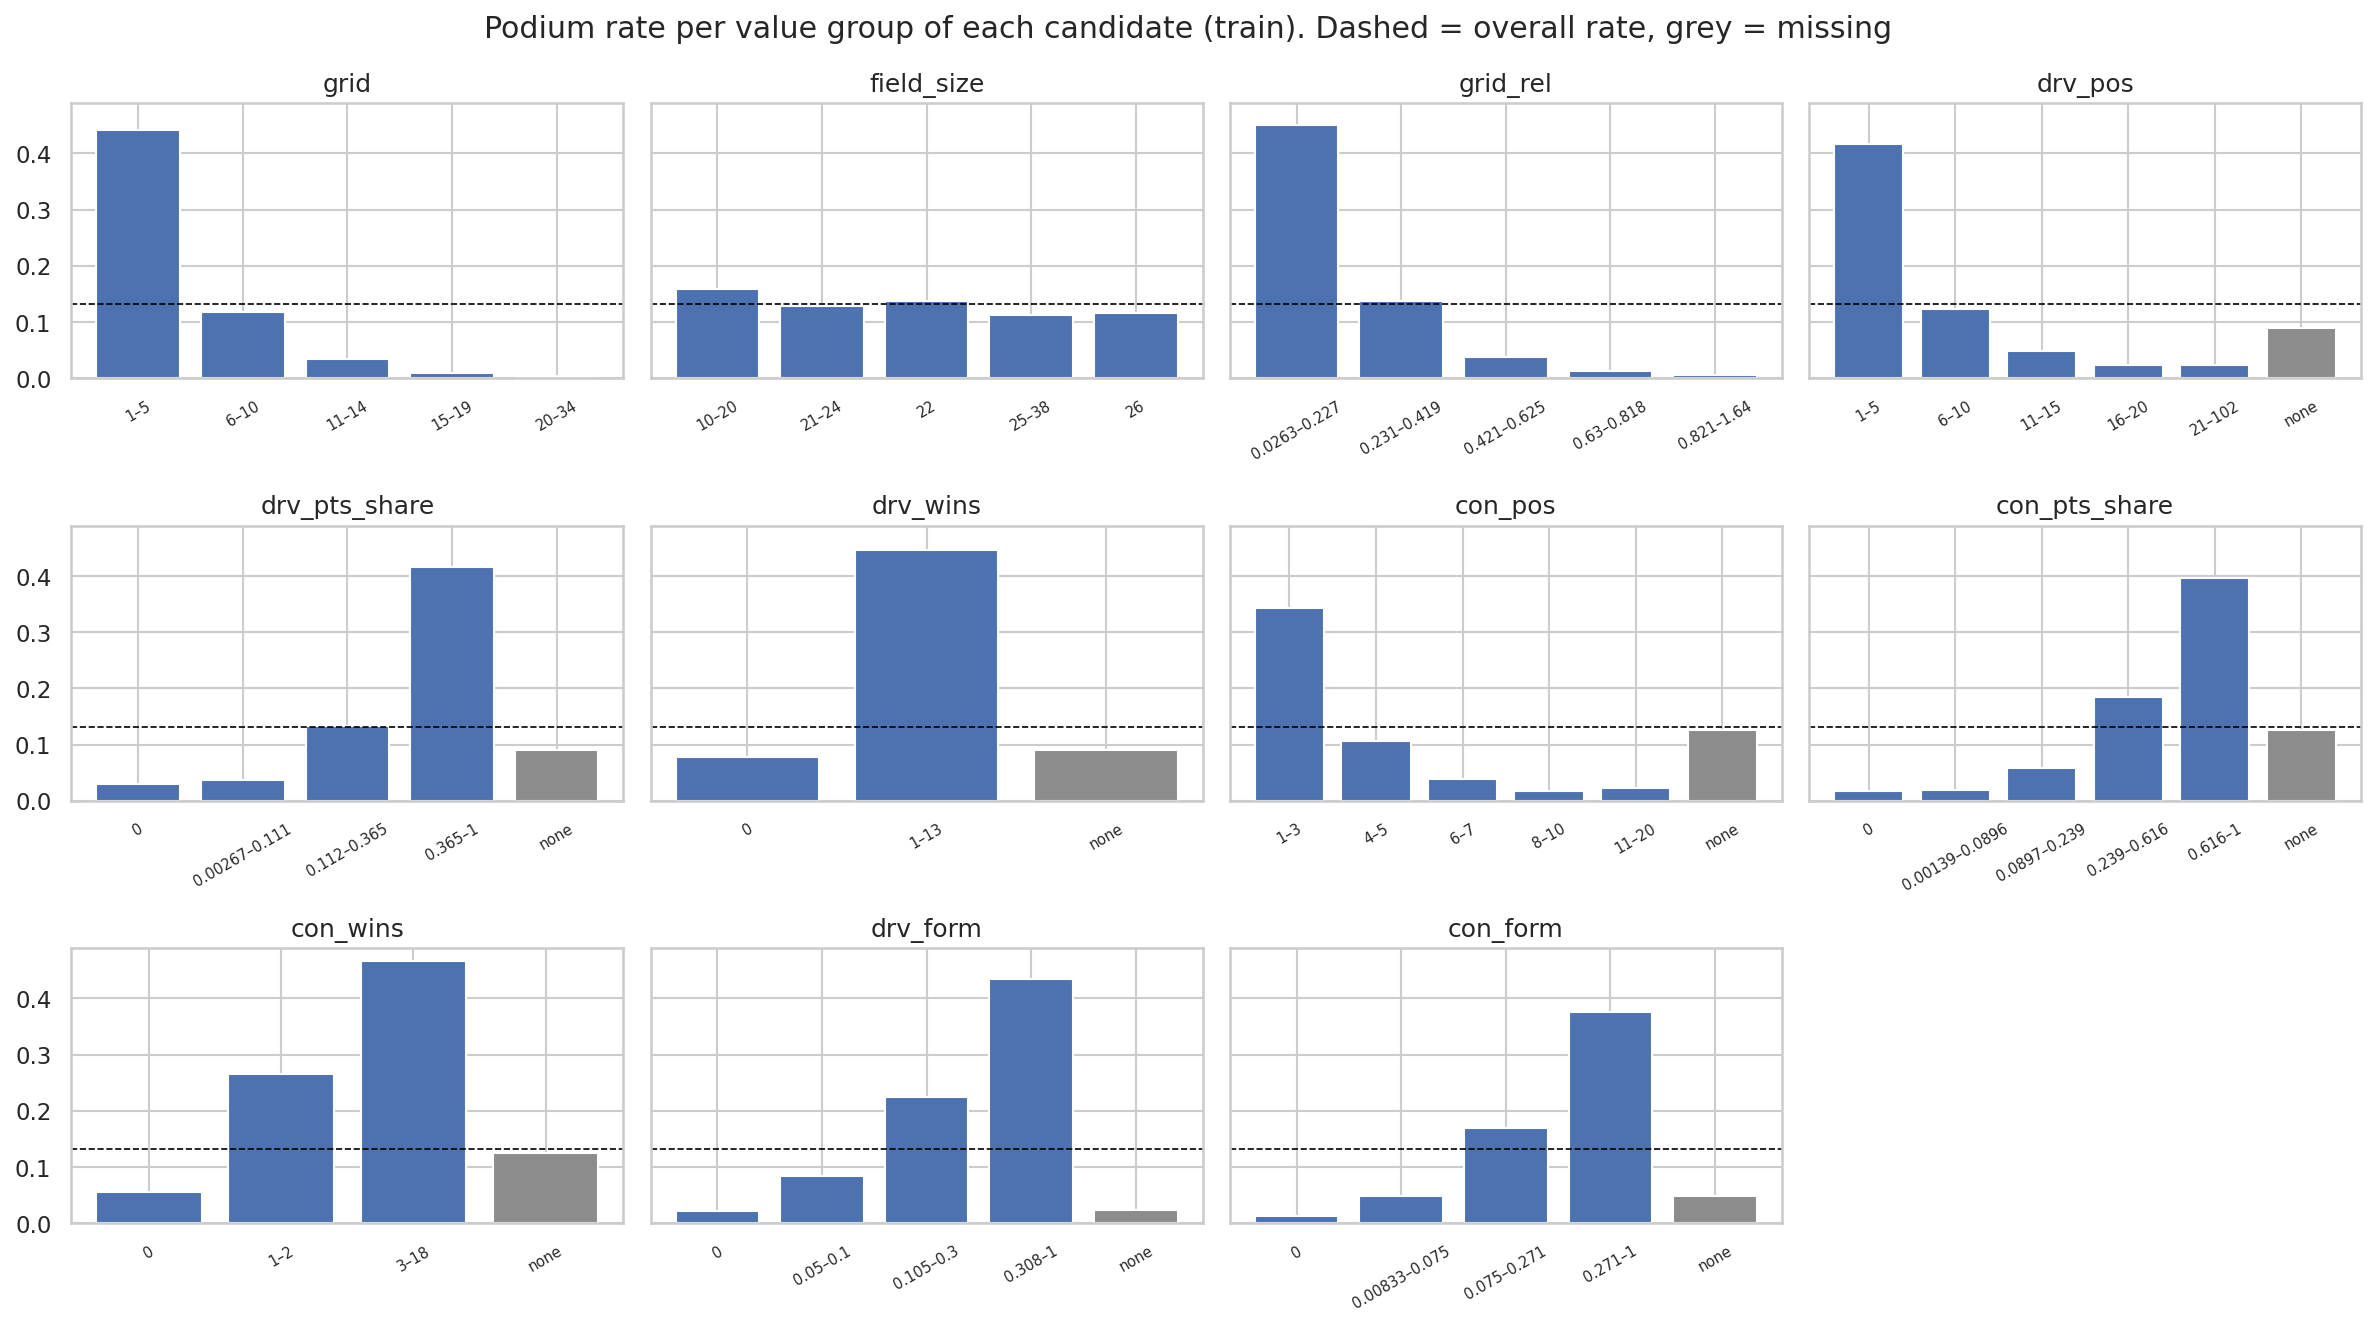
\includegraphics[width=\linewidth]{fig_12_feature_fifths.png}
\caption{Podium rate per value group of each candidate (train). Dashed = overall rate; grey = missing value.}
\label{fig:fifths}
\end{figure}

\begin{figure}[H]
\centering
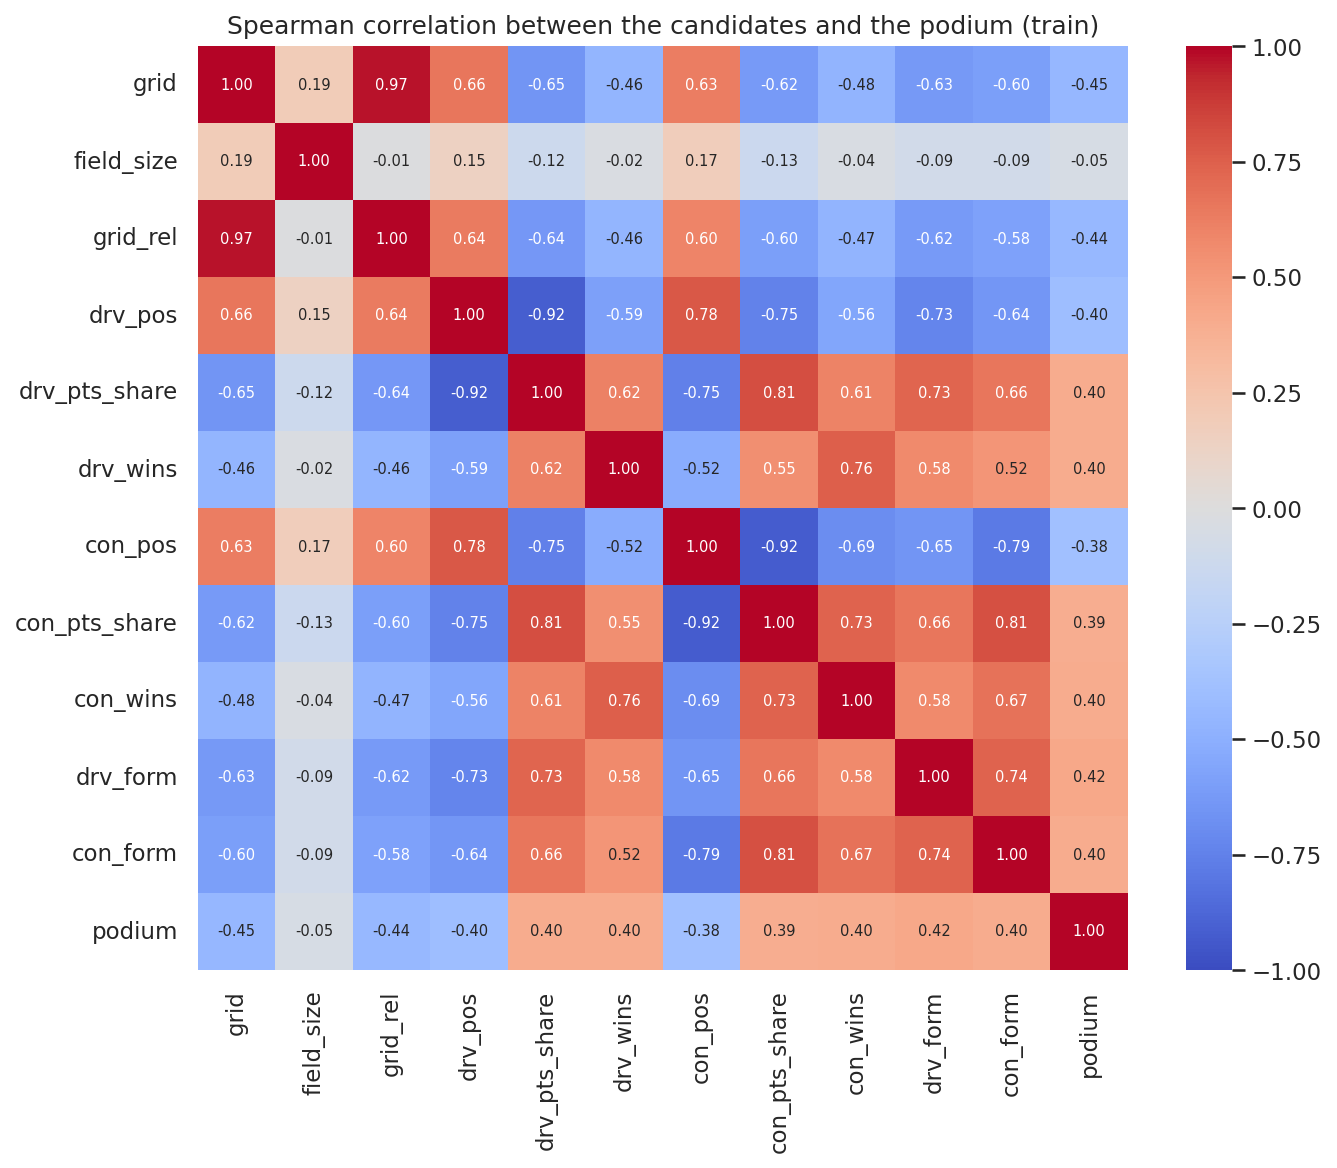
\includegraphics[width=0.66\linewidth]{fig_13_feature_corr.png}
\caption{Spearman correlation between the candidates and the podium (train; last row and column = podium).}
\label{fig:corr}
\end{figure}

Spearman correlation with the podium (train): \code{grid} $-0.449$, \code{grid\_rel} $-0.444$, \code{drv\_form} $0.422$, \code{drv\_wins} $0.404$, \code{con\_form} $0.403$, \code{drv\_pts\_share} $0.400$, \code{drv\_pos} $-0.400$, \code{con\_wins} $0.400$, \code{con\_pts\_share} $0.393$, \code{con\_pos} $-0.383$, \code{field\_size} $-0.052$.
All but field size are strong on their own, but many repeat each other (grid and relative grid, position and points share, driver and team standings, form and standings), so the plots alone cannot settle the list.

\subsection{Empirical selection: adding one group at a time}
Starting from \code{grid} only (the baseline), the groups are added one at a time in the order of \tab{tab:candidates}. Logistic regression and a random forest are retrained with fixed settings, so only the features change. \textbf{A group is kept if validation PR-AUC rises by at least 0.005 for both models}; a dropped group is never carried along. An extra group makes the models harder to explain and gives them more ways to fit noise, so it has to bring a gain worth having; 0.005 is that bar, and the bootstrap below checks it.

\begin{table}[H]
\centering\small
\caption{Feature-selection steps (validation PR-AUC) \nb{11.2}.}
\label{tab:ladder}
\begin{tabular}{llrrl}
\toprule
Step & Groups in this step & LR & RF & Decision \\
\midrule
grid & grid & 0.668 & 0.668 & start \\
+ field size & grid + field size & 0.668 & 0.668 & dropped \\
+ driver standings & grid + driver standings & 0.714 & 0.723 & \textbf{kept} \\
+ team standings & grid + driver + team standings & 0.706 & 0.704 & dropped \\
+ recent form & grid + driver standings + form & 0.716 & 0.730 & dropped \\
\midrule
all 11 candidates & & 0.719 & 0.720 & for comparison \\
\bottomrule
\end{tabular}
\end{table}

\begin{figure}[H]
\centering
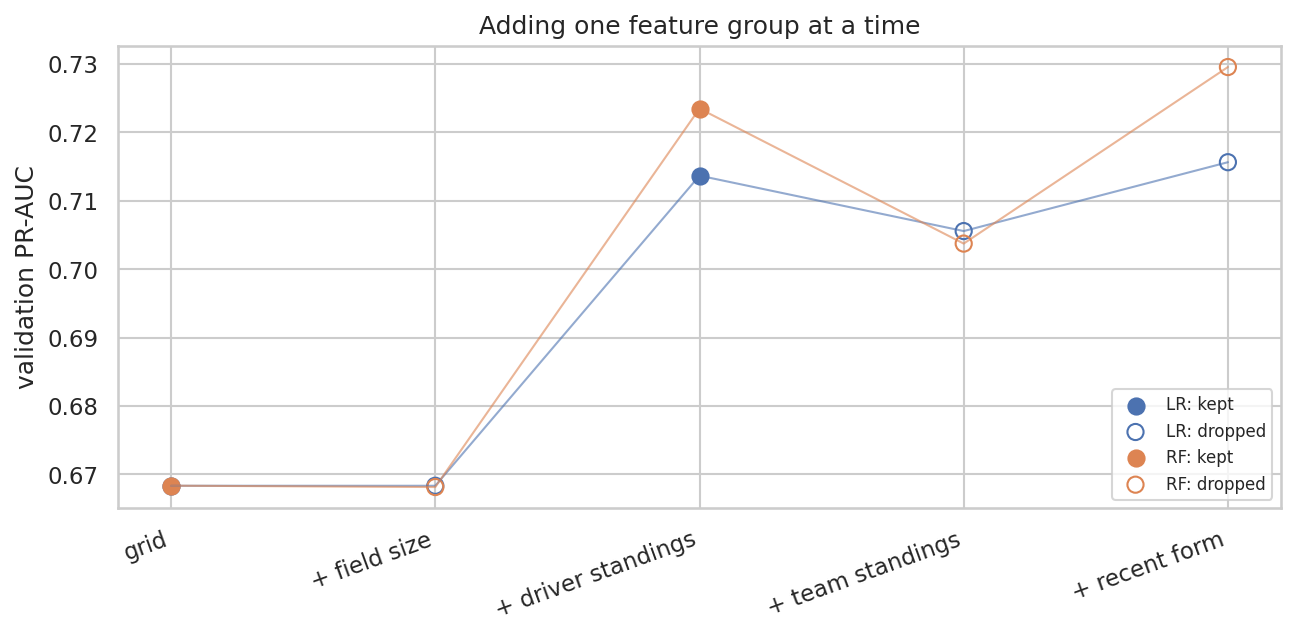
\includegraphics[width=0.8\linewidth]{fig_14_feature_ladder.png}
\caption{Validation PR-AUC as groups are added (filled = kept, open = dropped).}
\label{fig:ladder}
\end{figure}

\paragraph{Selected features (4):} \code{grid}, \code{drv\_pos}, \code{drv\_pts\_share}, \code{drv\_wins}.
Driver standings are the only group that clears the bar: how the driver is doing \emph{this season} is the strongest addition to where they start. Field size adds nothing; team standings make both models worse ($-0.008$, $-0.020$); recent form helps the forest a little ($+0.006$) but not logistic regression ($+0.002$), and the rule asks for both. All 11 candidates together change the score by $+0.005$ (LR) and $-0.003$ (RF) compared with the selected four, so seven more columns are not clearly better.
The result can depend on the order of the groups, and a dropped group is not tried again; the all-candidates row and the ablation (Section~\ref{sec:ablation}) are the checks on that.

\subsection{Statistical check of the selection}

\paragraph{Redundancy.} The variance inflation factor (VIF) of a column is $1/(1-R^2)$, where $R^2$ says how well the other columns predict it; above about 5 a column is mostly a copy. With all 11 candidates, \code{grid} (62.7) and \code{grid\_rel} (59.5) are copies of each other, and the points shares of the driver (6.4) and the team (7.2) mostly repeat the other standings columns. The selected four have VIFs of 1.6--3.5. All Spearman $p$-values are below 0.001, but with 22{,}000 rows even $\rho = -0.05$ is ``significant'', so the size of the correlation and the redundancy decide, not the $p$-value.

\paragraph{Each step against chance.} The same 2{,}000 bootstrap redraws of the validation races as in Section~\ref{sec:window} are used: both versions of each step are rescored on the same drawn rows (no retraining).

\begin{table}[H]
\centering\small
\caption{Change in validation PR-AUC for each step, with its 95\% bootstrap range \nb{11.2b}.}
\label{tab:selboot}
\begin{tabular}{llrrl}
\toprule
Step & Model & Change & 95\% range & 0.005 rule \\
\midrule
+ field size & LR / RF & $+0.000$ / $-0.000$ & $0.000$ to $0.000$ / $-0.001$ to $+0.000$ & dropped \\
+ driver standings & LR & $+0.045$ & $+0.009$ to $+0.085$ & \textbf{kept} \\
 & RF & $+0.055$ & $+0.017$ to $+0.093$ & \textbf{kept} \\
+ team standings & LR & $-0.008$ & $-0.020$ to $+0.004$ & dropped \\
 & RF & $-0.020$ & $-0.040$ to $+0.002$ & dropped \\
+ recent form & LR & $+0.002$ & $-0.023$ to $+0.029$ & dropped \\
 & RF & $+0.006$ & $-0.016$ to $+0.030$ & dropped \\
\bottomrule
\end{tabular}
\end{table}

The bootstrap agrees with the 0.005 rule at every step: only the kept step has a range above 0 for both models, and every dropped step has a range that includes 0.

%==============================================================================
\section{Preprocessing}\label{sec:prep}

\begin{enumerate}
\item \textbf{Imputation} with the \textbf{median} of the training rows (\code{SimpleImputer}). The columns with gaps are skewed (skew 1.0--4.5 for all but \code{con\_pos}; 56--84\% of rows lie at or below the mean), so the mean is pulled up by a few strong drivers and is a value hardly anyone has, while the median is what a typical driver has (\fig{fig:median}). Fill values: \code{grid} 12, \code{drv\_pos} 12, \code{drv\_pts\_share} 0.076, \code{drv\_wins} 0.
\item \textbf{Scaling} with \code{StandardScaler} (mean 0, standard deviation 1), so large numbers (grid 1--34, positions up to 102) do not dominate small ones (shares 0--1). It matters for logistic regression and the network; the forest does not care, but every model gets the same inputs.
\end{enumerate}
Both steps are fit on the \textbf{training seasons only} and applied unchanged to validation and test. No row is dropped for a missing value: 68 of the 1{,}359 test rows (5.0\%) have missing standings and all are scored. Scaling only shifts and stretches the values (\fig{fig:scaling}). Validation and test are not refit, so their means differ from 0 (for example \code{grid} $-0.22$ and $-0.23$), which shows how the newer seasons differ from the training seasons.

\begin{figure}[H]
\centering
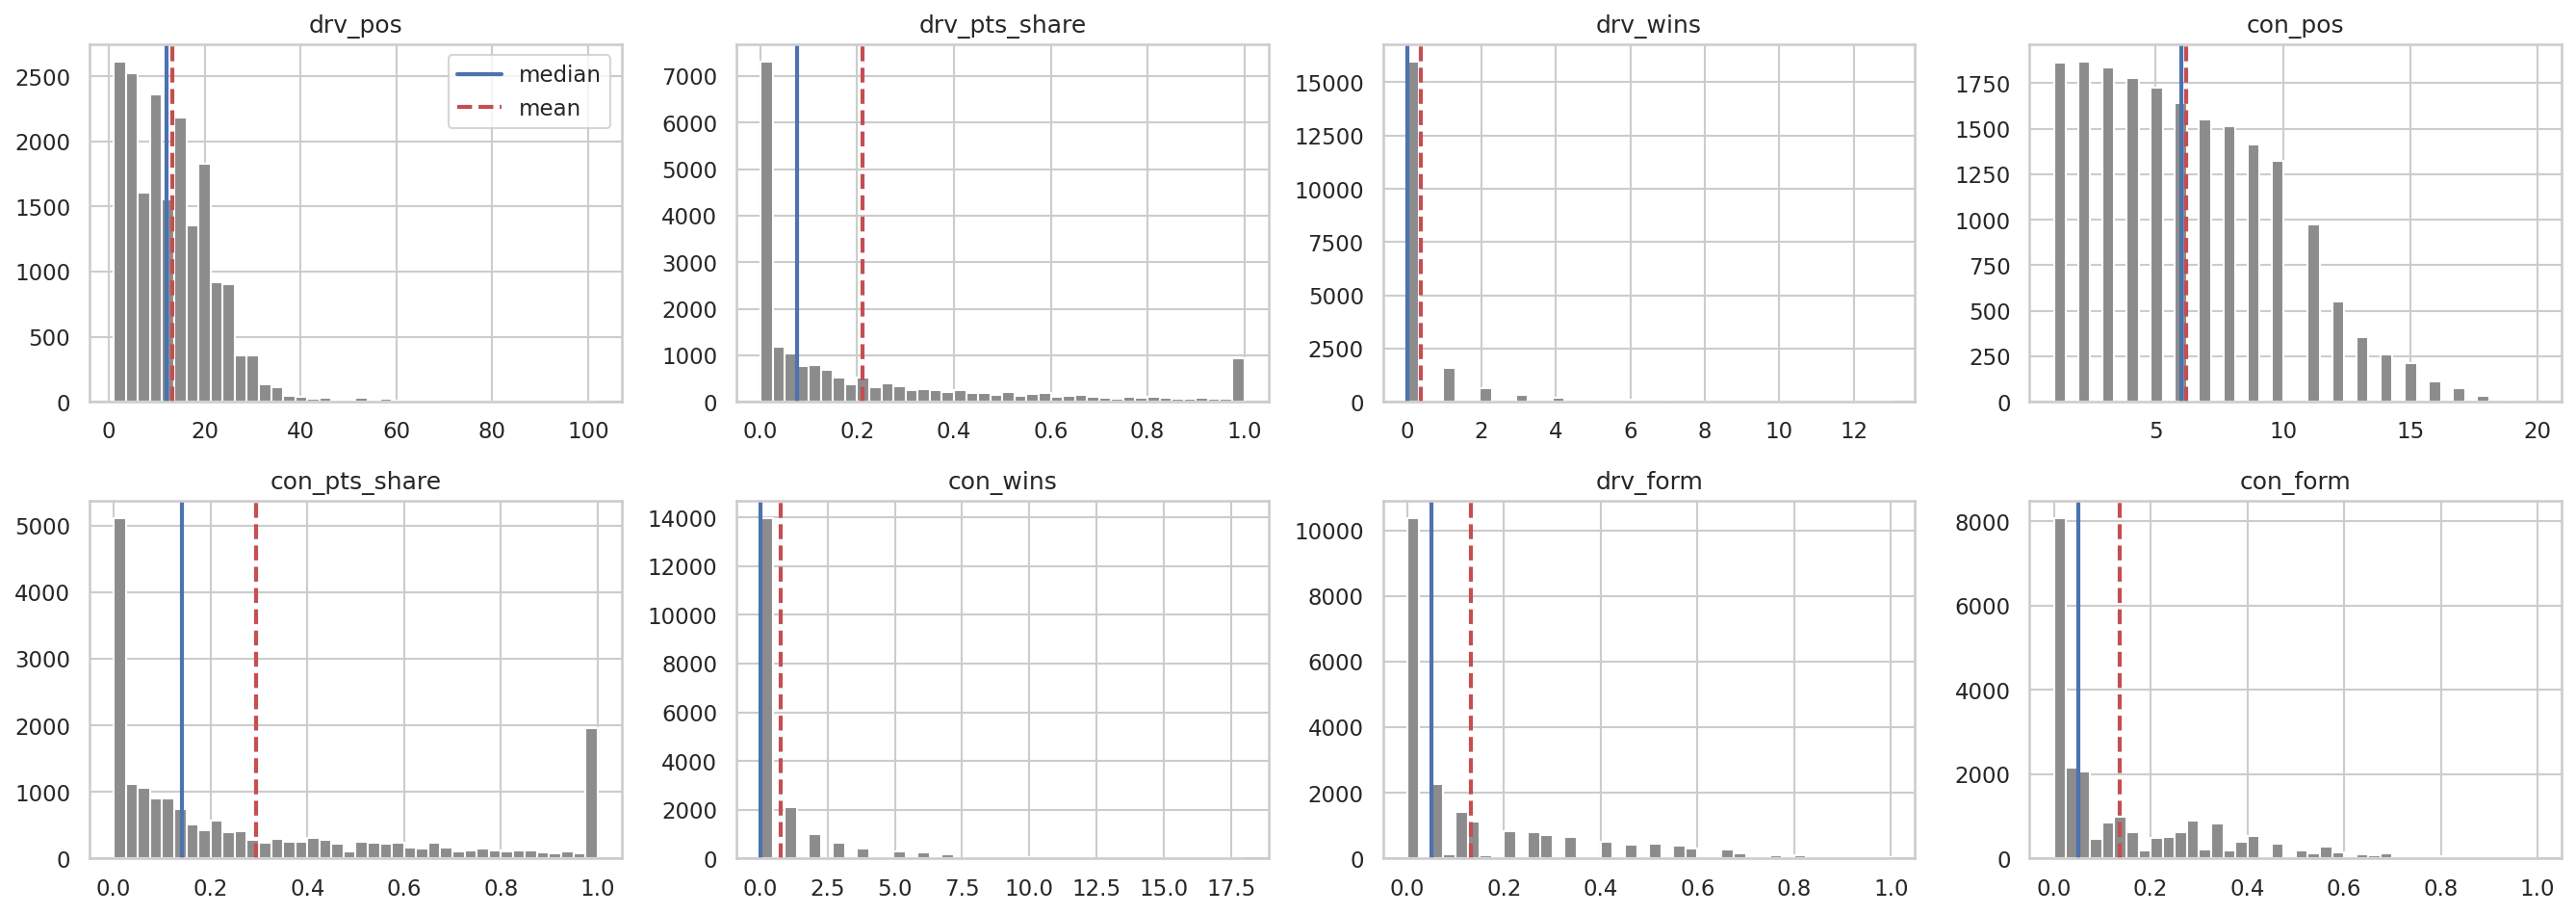
\includegraphics[width=\linewidth]{fig_11d_median_vs_mean.png}
\caption{The training columns with gaps; solid = median (the fill value), dashed = mean.}
\label{fig:median}
\end{figure}

\begin{figure}[H]
\centering
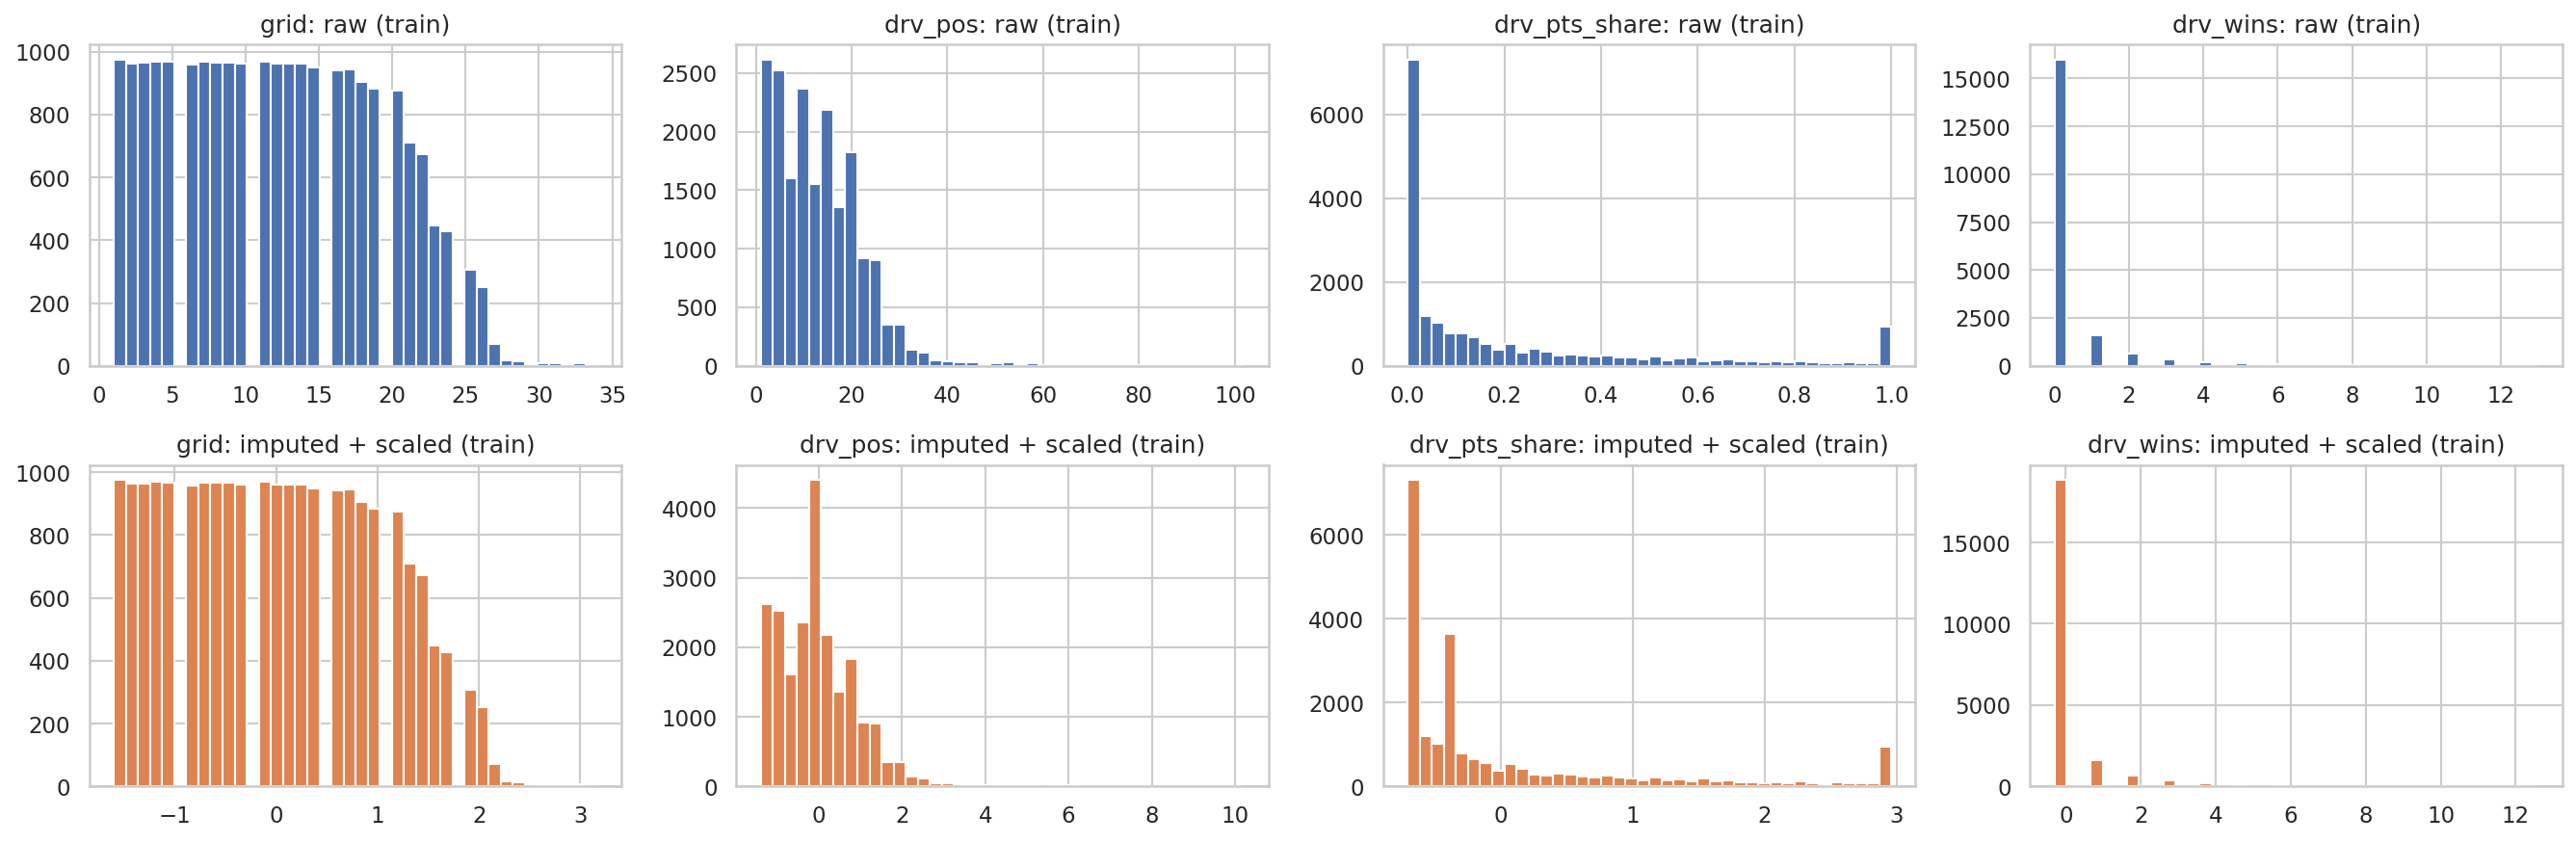
\includegraphics[width=\linewidth]{fig_15_scaling.png}
\caption{The four chosen features on train, raw (top) and after imputing and scaling (bottom).}
\label{fig:scaling}
\end{figure}

%==============================================================================
\section{Models}

All models use the same rows and the same four inputs, so their scores are directly comparable. No single model is picked as ``final''; all three are reported and explained alike.

\begin{itemize}
\item \textbf{Baseline: logistic regression on \code{grid} only}, the simplest reasonable model. The others must beat it to earn their complexity.
\item \textbf{Logistic regression:} a weighted sum of the inputs passed through a sigmoid. Easy to read, but it can only learn effects that keep going in one direction.
\item \textbf{Random forest}~\cite{breiman2001}: 300 decision trees, each on a random sample of rows and features, averaged. It learns curves and interactions, but is harder to read.
\item \textbf{Shallow neural network} (Keras): one or two hidden \code{Dense} ReLU layers, one sigmoid output, binary cross-entropy, Adam (learning rate 0.001), batches of 256, at most 200 epochs, early stopping on validation loss (patience 15, best weights kept). Flexible, but a black box that depends on scaling and random initialisation.
\end{itemize}

\paragraph{Tuning (validation only).} Every combination of class weight (none / \code{balanced}) and settings was trained, and the best validation PR-AUC kept (\tab{tab:tuning}). The threshold of each model is the one with the best F1 on validation: baseline 0.427, logistic regression 0.399, random forest 0.432, network 0.348.

\begin{table}[H]
\centering\small
\caption{Tuning (validation PR-AUC). Chosen settings in bold.}
\label{tab:tuning}
\begin{tabular}{llrr}
\toprule
Model & Settings & No class weight & Balanced \\
\midrule
LR & $C = 0.01$ / 0.1 / 1 / 10 & 0.711 / 0.714 / 0.714 / \textbf{0.714} & 0.711 / 0.711 / 0.711 / 0.711 \\
RF & depth 4, min leaf 20 / 50 & 0.722 / 0.715 & 0.715 / 0.708 \\
RF & depth 6, min leaf 20 / 50 & \textbf{0.723} / 0.720 & 0.722 / 0.717 \\
RF & depth 8, min leaf 20 / 50 & 0.722 / 0.718 & 0.723 / 0.719 \\
\bottomrule
\end{tabular}
\end{table}

\begin{table}[H]
\centering\small
\caption{Neural-network settings (validation).}
\label{tab:nn}
\begin{tabular}{lrrcrr}
\toprule
Setting & Epochs run & Best epoch & Stopped early & Best val loss & Val PR-AUC \\
\midrule
\textbf{(16)} & 200 & 187 & no & 0.2265 & \textbf{0.726} \\
(32) & 200 & 200 & no & 0.2252 & 0.726 \\
(32, 16) & 130 & 115 & yes & 0.2242 & 0.723 \\
(16) + dropout 0.2 & 102 & 87 & yes & 0.2325 & 0.716 \\
(32, 16) + dropout 0.2 & 60 & 45 & yes & 0.2276 & 0.721 \\
(16) + balanced & 200 & 200 & no & 0.4201 & 0.726 \\
\bottomrule
\end{tabular}
\end{table}

The best setting of each model uses no class weight. $C$ barely matters for logistic regression. The three network sizes without dropout are within 0.003 of each other and the smallest (16 units) scores highest, so it is kept: with four inputs a bigger network gains nothing (\fig{fig:nnloss}).

\begin{figure}[H]
\centering
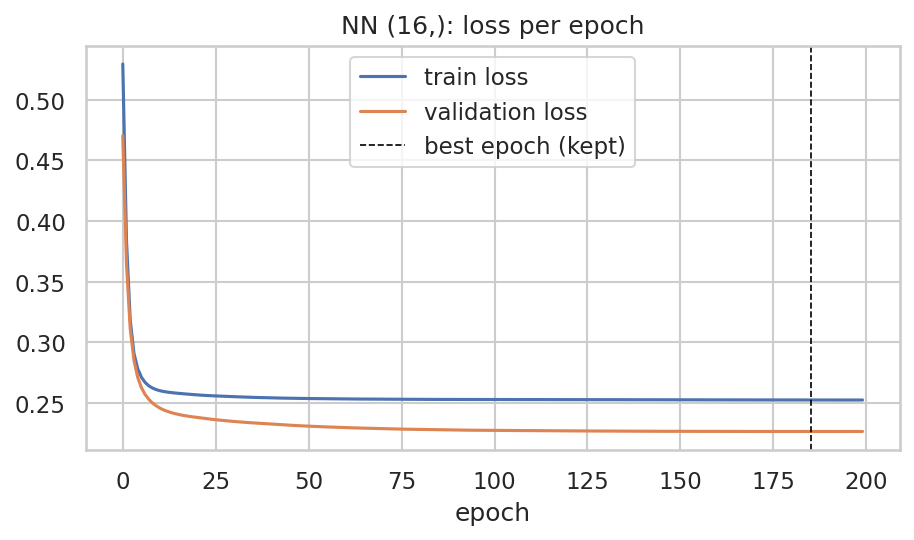
\includegraphics[width=0.55\linewidth]{fig_16_nn_loss.png}
\caption{Network (16): training and validation loss per epoch; dashed = the epoch whose weights are kept.}
\label{fig:nnloss}
\end{figure}

%==============================================================================
\section{Results}

\begin{table}[H]
\centering\small
\caption{All metrics on train, validation and the unseen test seasons. Thresholds were chosen on validation \nb{14}.}
\label{tab:results}
\begin{tabular}{llrrrrrr}
\toprule
Model & Set & PR-AUC & ROC-AUC & F1 & Precision & Recall & Accuracy \\
\midrule
Baseline (LR on grid) & train & 0.487 & 0.883 & 0.534 & 0.533 & 0.535 & 0.877 \\
 & val & 0.668 & 0.918 & 0.712 & 0.712 & 0.712 & 0.914 \\
 & test & 0.647 & 0.914 & 0.649 & 0.650 & 0.647 & 0.895 \\
\midrule
Logistic regression & train & 0.545 & 0.892 & 0.535 & 0.565 & 0.507 & 0.883 \\
 & val & 0.714 & 0.928 & 0.709 & 0.702 & 0.716 & 0.912 \\
 & test & 0.708 & 0.930 & 0.678 & 0.690 & 0.667 & 0.905 \\
\midrule
Random forest & train & 0.567 & 0.901 & 0.543 & 0.586 & 0.505 & 0.888 \\
 & val & 0.723 & 0.939 & 0.720 & 0.715 & 0.724 & 0.915 \\
 & test & 0.720 & 0.940 & 0.668 & 0.709 & 0.632 & 0.906 \\
\midrule
Neural network & train & 0.549 & 0.896 & 0.566 & 0.517 & 0.626 & 0.873 \\
 & val & 0.726 & 0.936 & 0.716 & 0.655 & 0.790 & 0.906 \\
 & test & 0.706 & 0.938 & 0.681 & 0.614 & 0.765 & 0.893 \\
\bottomrule
\end{tabular}
\end{table}

\begin{figure}[H]
\centering
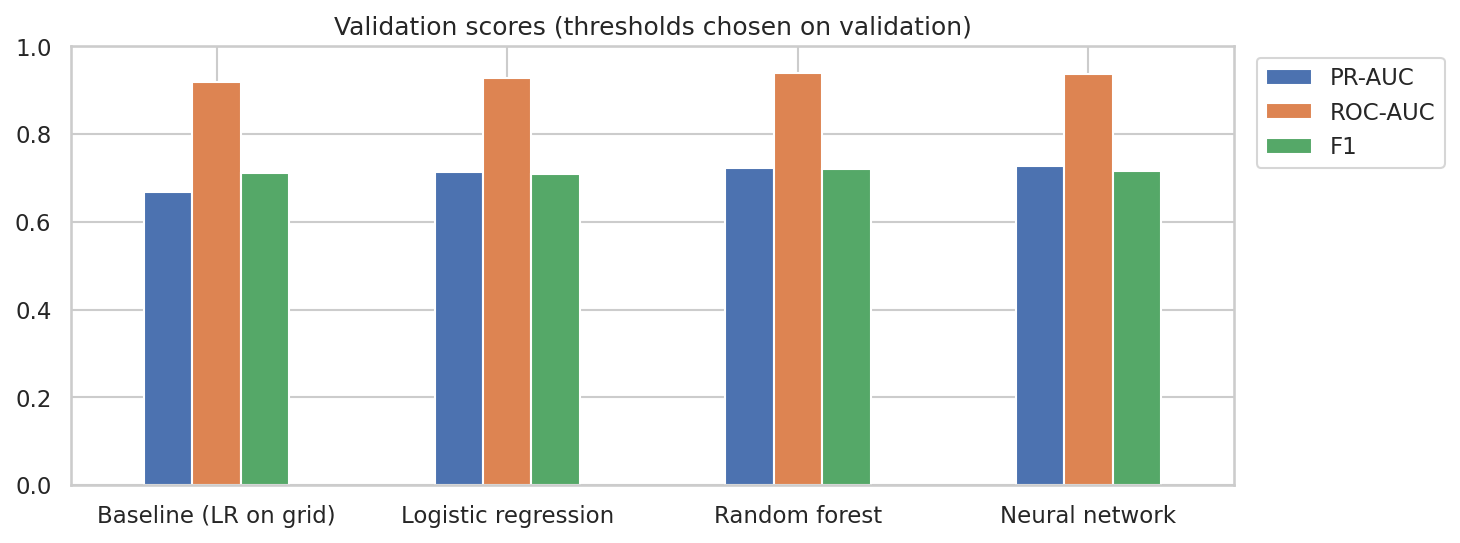
\includegraphics[width=0.49\linewidth]{fig_17_models_val.png}\hfill
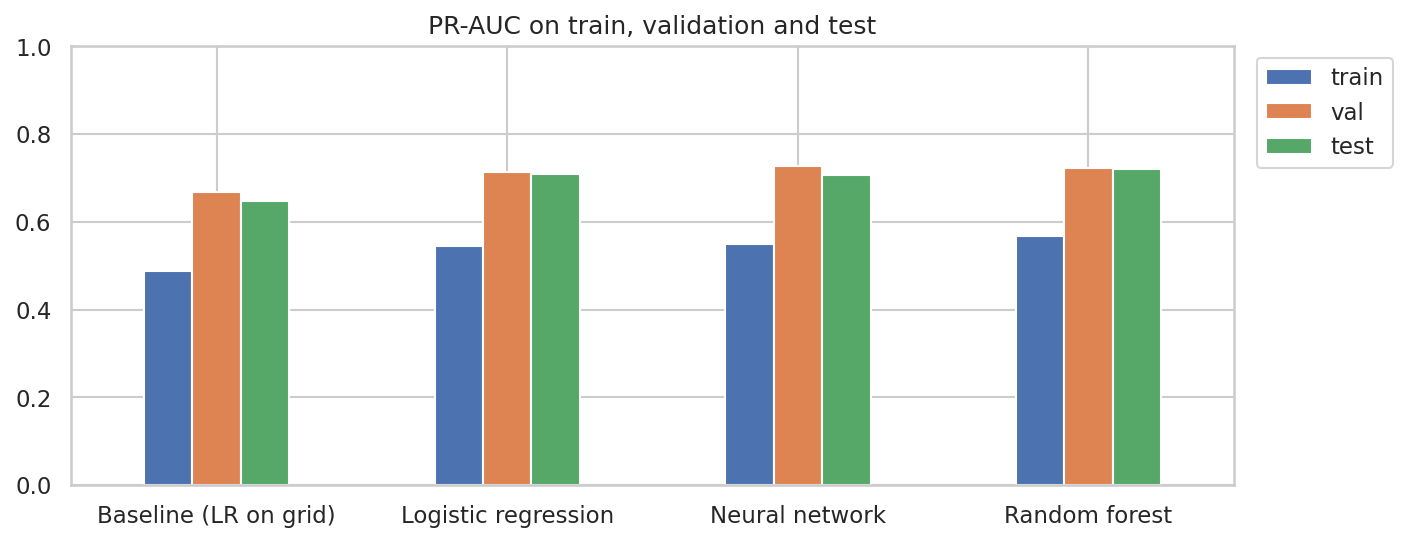
\includegraphics[width=0.49\linewidth]{fig_18_pr_auc_splits.png}
\caption{Left: validation PR-AUC, ROC-AUC and F1. Right: PR-AUC on train, validation and test.}
\label{fig:results}
\end{figure}

\begin{figure}[H]
\centering
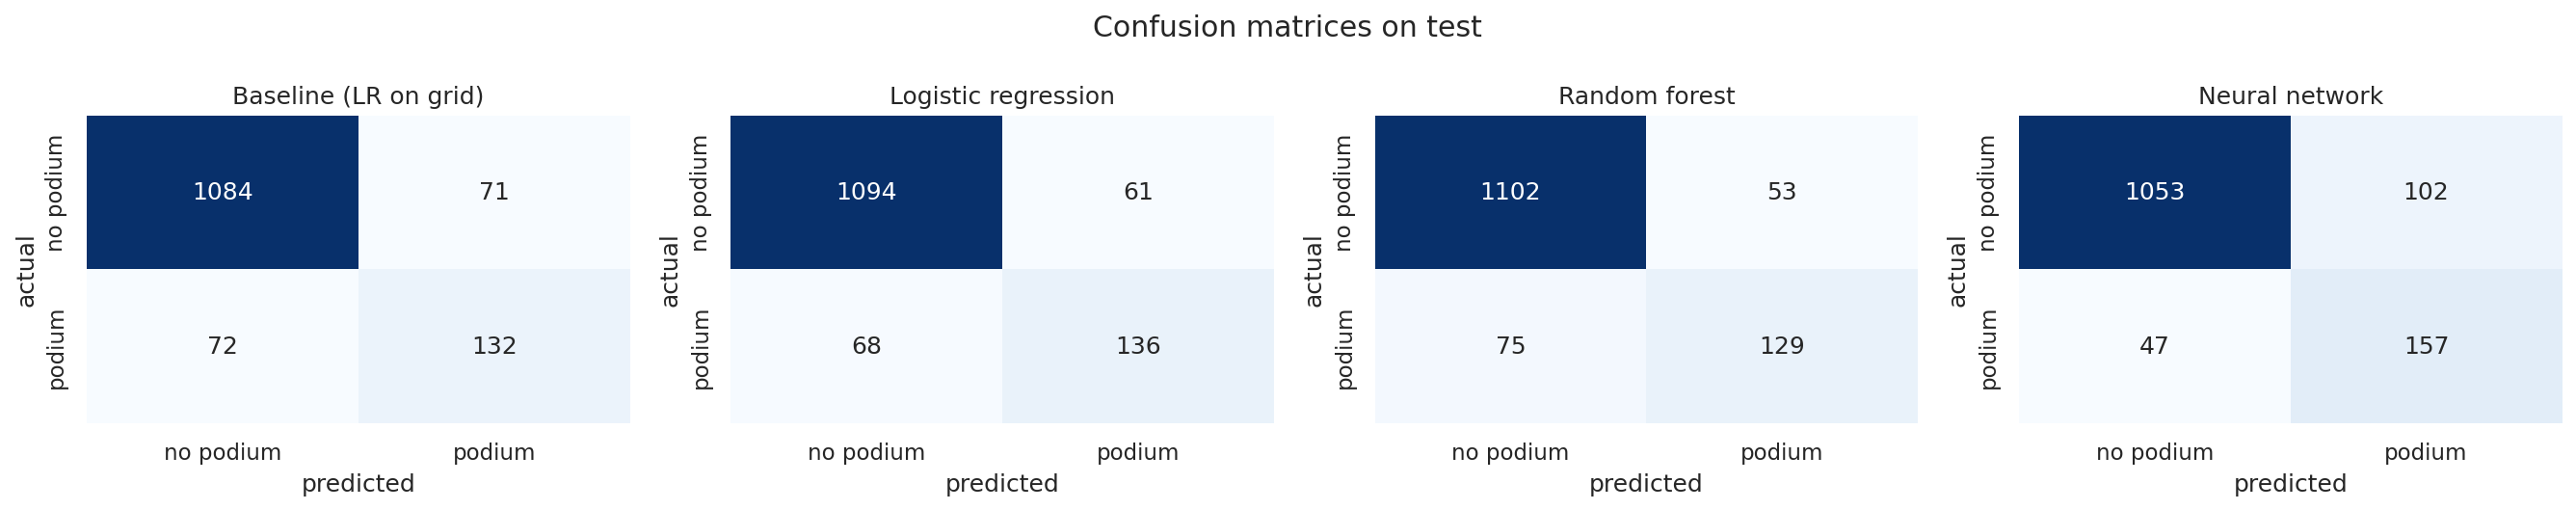
\includegraphics[width=\linewidth]{fig_19_confusion_test.png}
\caption{Confusion matrices on the test seasons (rows = actual, columns = predicted).}
\label{fig:cm}
\end{figure}

\paragraph{Reading the results.}
\begin{itemize}
\item \textbf{All three models beat the baseline} on validation and test. On test, PR-AUC rises from 0.647 to 0.706--0.720 and ROC-AUC from 0.914 to 0.930--0.940: adding the driver's season standings to the grid earns its complexity.
\item \textbf{The three models are about equally good.} The network is first on validation (0.726), the forest on test (0.720), and the gaps are about 0.01, which a few hundred podiums cannot separate. Test scores are within 0.02 of validation.
\item The network has the highest test recall (0.77) and the lowest precision (0.61), because its threshold (0.348) is the lowest; F1 is 0.67--0.68 for all three.
\item \textbf{Train is lower than validation} (PR-AUC 0.55--0.57 vs.\ 0.71--0.73), which is neither under- nor overfitting. Split by era \nb{13.1}, train PR-AUC is 0.41--0.47 in 1950--1979 but 0.69--0.77 in 2014--2017, close to validation, while the podium rate is about the same in each era (13--14\%). The old races are simply harder to predict.
\item \textbf{The outputs are on the right scale:} every model's average prediction on validation (0.149--0.159) is close to the real rate (0.150), and none of the chosen settings uses \code{balanced} weights.
\end{itemize}

%==============================================================================
\section{Experiments}

Every experiment retrains all three models with their chosen settings, so only the tested thing changes.

\subsection{Feature-group ablation}\label{sec:ablation}
One group at a time is removed and the models are retrained. This is done from the selected features (what each kept group contributes) and from all 11 candidates (so every group gets a result). Test drops are only reported.

\begin{table}[H]
\centering\small
\caption{Drop in PR-AUC when a group is removed (validation / test). Negative = better without it.}
\label{tab:ablation}
\begin{tabular}{llrrr}
\toprule
From & Removed group & Logistic regression & Random forest & Neural network \\
\midrule
selected 4 & grid & 0.078 / 0.143 & 0.092 / 0.161 & 0.097 / 0.143 \\
 & driver standings & 0.045 / 0.061 & 0.055 / 0.073 & 0.058 / 0.059 \\
\midrule
all 11 & grid & $-0.001$ / $-0.002$ & $-0.003$ / 0.010 & 0.007 / 0.008 \\
 & field size & 0.001 / 0.001 & 0.005 / 0.013 & 0.027 / 0.024 \\
 & driver standings & 0.009 / 0.007 & 0.006 / 0.003 & $-0.001$ / $-0.001$ \\
 & team standings & 0.004 / $-0.001$ & $-0.013$ / $-0.000$ & $-0.002$ / 0.005 \\
 & recent form & 0.013 / 0.011 & 0.003 / 0.004 & 0.015 / 0.002 \\
\bottomrule
\end{tabular}
\end{table}

\begin{figure}[H]
\centering
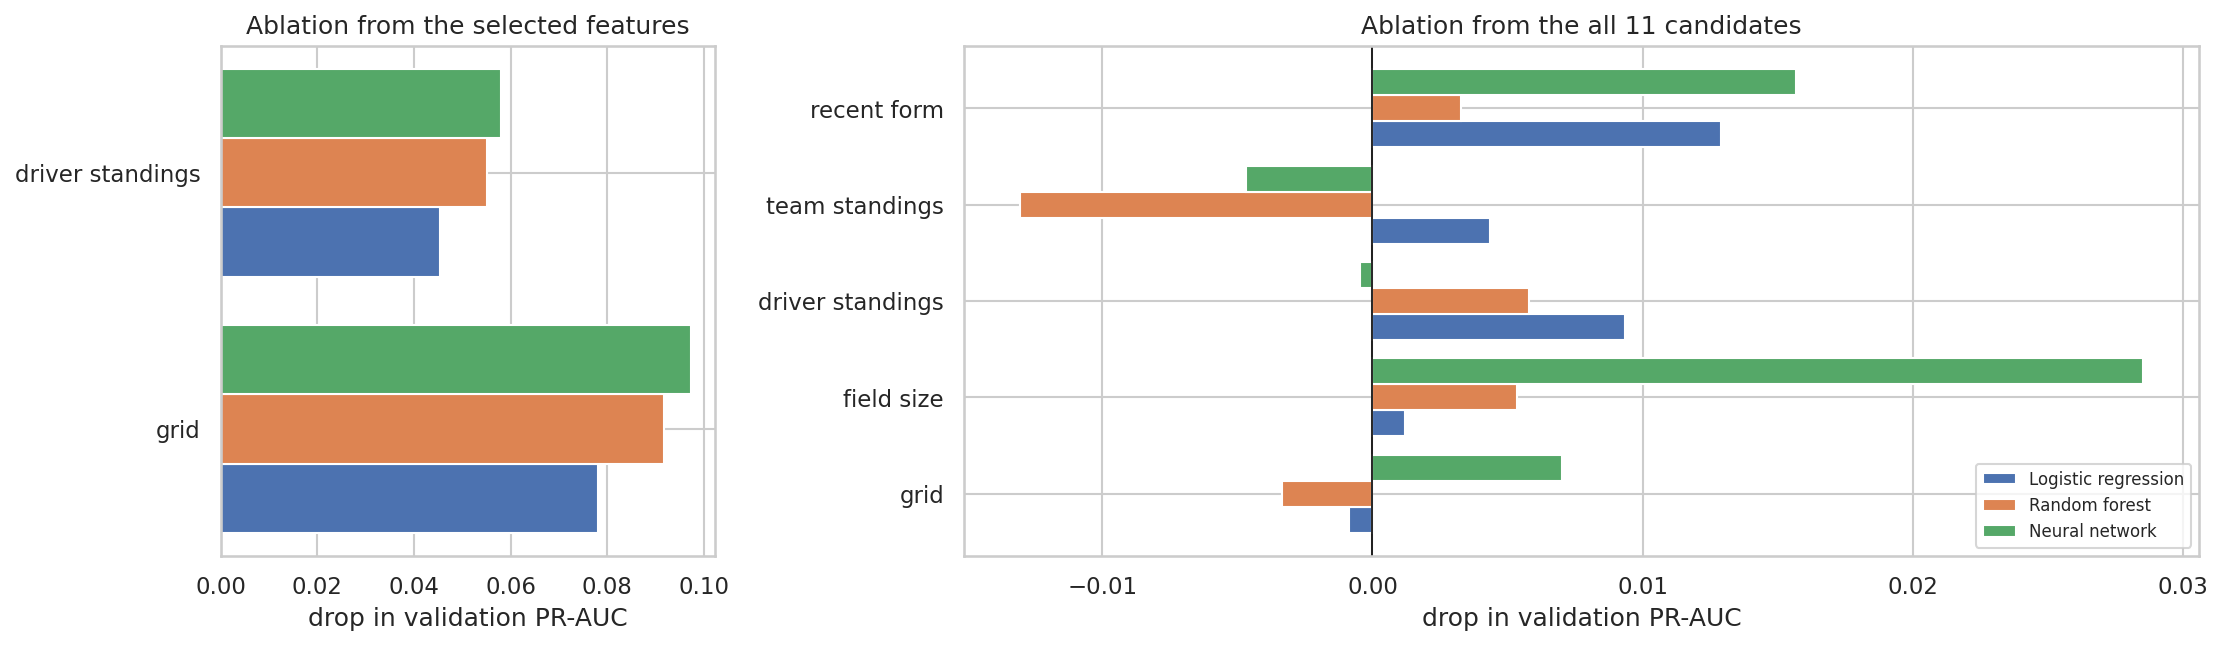
\includegraphics[width=\linewidth]{fig_20_ablation.png}
\caption{Drop in validation PR-AUC per removed group; left from the selected features, right from all 11 candidates.}
\label{fig:ablation}
\end{figure}

\textbf{Reading.} From the selected features, removing the grid costs the most (0.08--0.10 on validation, 0.14--0.16 on test) and removing the driver standings costs 0.05--0.06 on validation and 0.06--0.07 on test, so both kept groups help after training too. From all 11 candidates every removal costs little (at most 0.027) and several make a model better: even removing the grid costs almost nothing, because \code{grid\_rel} carries nearly the same information. The groups repeat each other, which is why only two were kept.

\subsection{Preprocessing experiments}

\begin{table}[H]
\centering\small
\caption{Preprocessing experiments (validation PR-AUC) \nb{15.2}.}
\label{tab:order}
\begin{tabular}{lrrr}
\toprule
Version & LR & RF & NN \\
\midrule
\textbf{Used:} fit on train only, impute $\rightarrow$ scale, median & 0.7137 & 0.7234 & 0.7263 \\
1. Fit on all seasons (leaky) & 0.7138 & 0.7229 & 0.7248 \\
2. Scale $\rightarrow$ impute & 0.7138 & 0.7234 & 0.7268 \\
3a. Mean instead of median & 0.7150 & 0.7227 & 0.7252 \\
3b. Median + ``was missing'' flag & 0.7170 & 0.7238 & 0.7281 \\
\bottomrule
\end{tabular}
\end{table}

\begin{itemize}
\item \textbf{Experiment 1 (before or after splitting):} fitting the imputer and scaler on all seasons is leakage, but it changes PR-AUC by at most 0.0015, because 88\% of all rows are training rows, so the statistics hardly move. Fitting on train only is still the correct order: it is the only one possible for a real future race.
\item \textbf{Experiment 2 (impute or scale first):} at most $+0.0005$. The filled value is the same point either way; imputing first is kept so the scaler sees exactly the data the model gets.
\item \textbf{Experiment 3 (fill value):} the mean is no better ($+0.0013$, $-0.0007$, $-0.0011$). The missing flag is slightly better for all three models ($+0.0032$, $+0.0004$, $+0.0018$), but every gain is below the 0.005 bar, so the plain median stays and the models keep four inputs.
\end{itemize}

\subsection{Why not the window with the best validation score?}\label{sec:formtest}
Section~\ref{sec:window} uses the shortest window that validation cannot tell apart from the best one (20 races) instead of the best one itself (75 races). This section shows what the longer window does on the test seasons; test is only reported, and nothing is chosen from it. \textbf{Hypothesis:} a long window remembers several seasons. The validation seasons were one stable era led by Mercedes (45\% of validation podiums), so a long memory predicted well there; with the new car rules of 2022 (general knowledge) the order at the front changed, and a long window kept ranking the old order first.

\begin{table}[H]
\centering\small
\caption{The window model (LR on grid + form) on validation and test; test is only reported.}
\label{tab:formtest}
\begin{tabular}{lrrrrrrrrrr}
\toprule
Window & 1 & 3 & 5 & 10 & \textbf{20} & 30 & 50 & 75 & 100 & 150 \\
\midrule
Val PR-AUC & 0.681 & 0.692 & 0.691 & 0.699 & 0.710 & 0.715 & 0.729 & 0.730 & 0.724 & 0.726 \\
Test PR-AUC & 0.663 & 0.702 & 0.695 & 0.710 & 0.710 & 0.697 & 0.680 & 0.658 & 0.633 & 0.603 \\
\bottomrule
\end{tabular}
\end{table}

\begin{figure}[H]
\centering
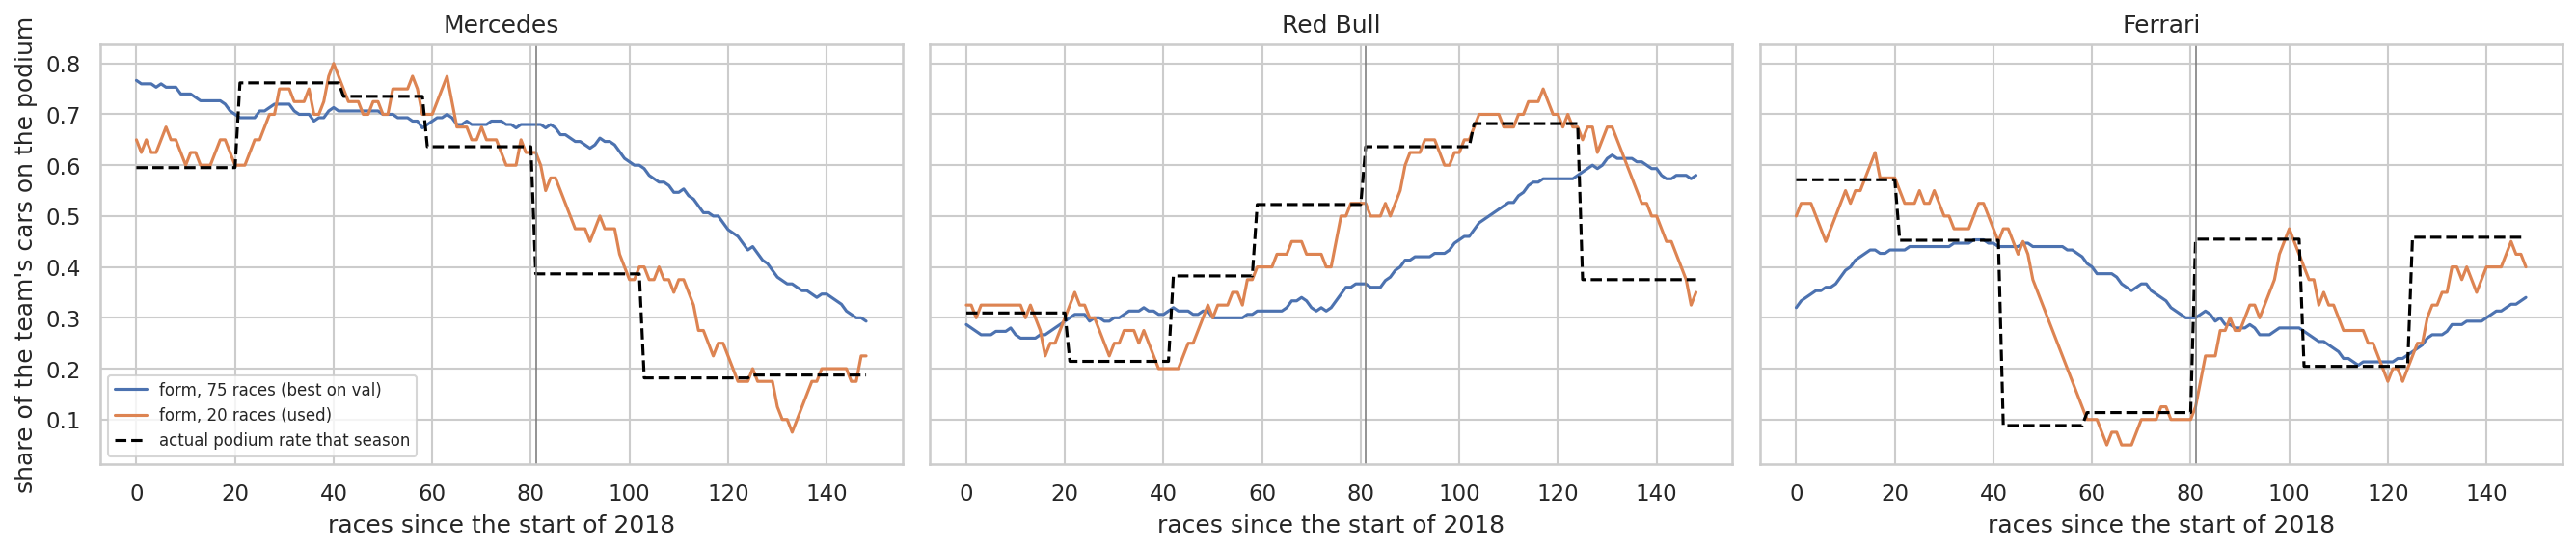
\includegraphics[width=\linewidth]{fig_21_form_window_test.png}
\caption{Team form of Ferrari, Mercedes and Red Bull from 2018, with 75 and 20 races, and the real podium rate of each season (dashed); grey line = first race of 2022.}
\label{fig:formtest}
\end{figure}

The long windows are best on validation but worst on test (0.658 for 75 races, 0.603 for 150, against 0.710 for 10--20). In 2022 the 75-race form still put Mercedes far ahead of Red Bull (0.65 against 0.41) while Red Bull's cars actually reached the podium more often (0.64 against 0.39); the 20-race form had already switched the order (0.59 against 0.49). The short window lags too, by about a season (Red Bull 0.54 in 2024 against a real 0.38). This fits the hypothesis, but it rests on three teams and three seasons.

%==============================================================================
\section{Explainability (XAI)}

\begin{center}
\fbox{\parbox{0.92\linewidth}{\textbf{Explanations are not causes.} An important feature is one the model \emph{relies on to make predictions}. It is not evidence that the feature \emph{causes} podium finishes. A front grid slot, for example, is mostly a sign of a fast car, and the fast car is what produces podiums. Inputs that overlap (the three standings columns) share the credit, and how they share it depends on the method.}}
\end{center}

\paragraph{Setup \nb{16}.} The brief asks for permutation importance and SHAP globally, and LIME and/or local SHAP for one row. We use SHAP's \textbf{permutation explainer}~\cite{lundberg2017} for all three models (the course staff confirmed this covers ``permutation importance''): it switches inputs off in random orders, replacing them with values from 100 training rows, and records how far the predicted probability moves. The forest is also explained with \code{TreeExplainer}, which computes the values exactly from the trees. SHAP values are in probability units and add up to \emph{prediction $-$ average prediction} (asserted within 0.005). The rows are validation rows (2018--2021), and the inputs are shown in their original units. The baseline has one input, so there is nothing to split.

\subsection{Global: SHAP summary plots}
\begin{figure}[H]
\centering
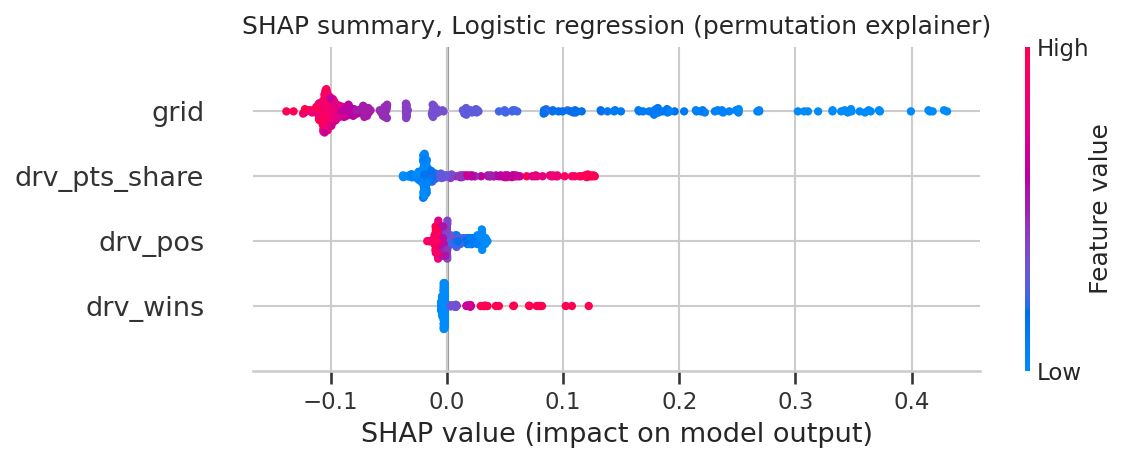
\includegraphics[width=0.49\linewidth]{fig_22_shap_summary_lr.png}\hfill
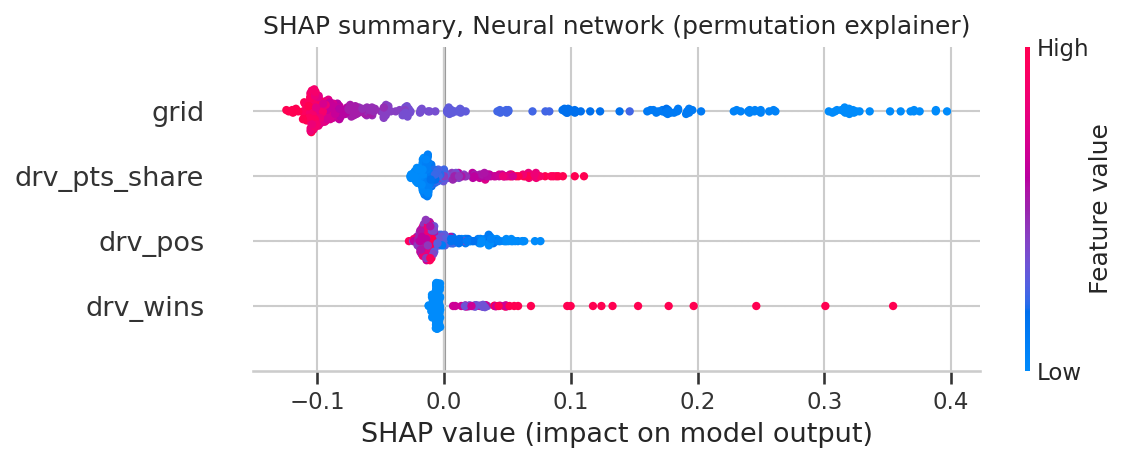
\includegraphics[width=0.49\linewidth]{fig_22_shap_summary_nn.png}\\[4pt]
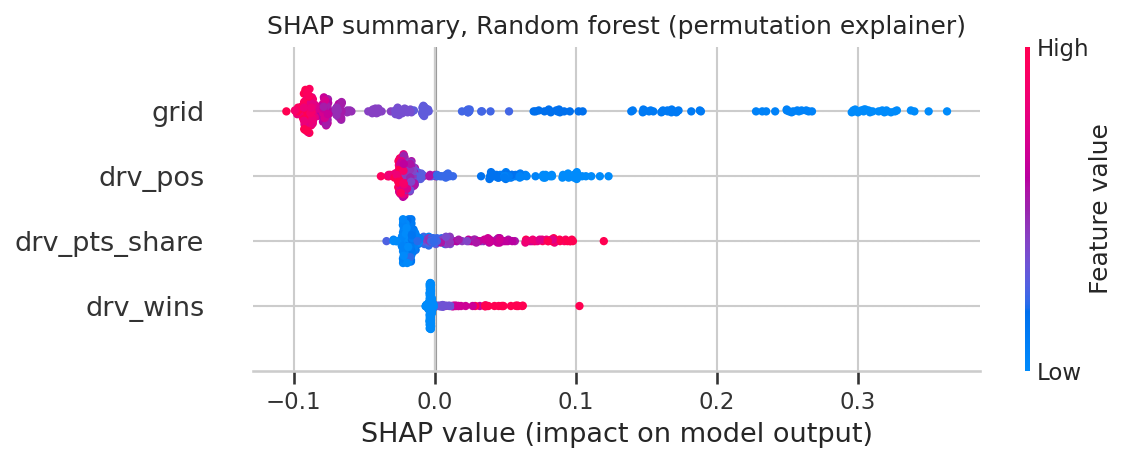
\includegraphics[width=0.49\linewidth]{fig_22_shap_summary_rf.png}\hfill
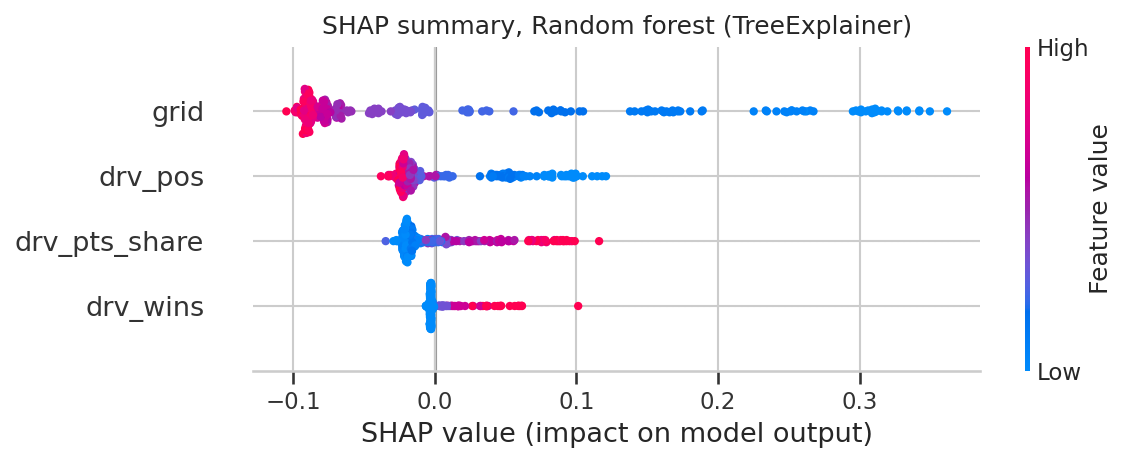
\includegraphics[width=0.49\linewidth]{fig_22_shap_summary_rf_tree.png}
\caption{SHAP summary plots on 300 validation rows: logistic regression and network (top), forest with the permutation explainer and with \code{TreeExplainer} (bottom). One dot per driver-race; right = higher podium probability; colour = the input's value (red high, blue low).}
\label{fig:shap}
\end{figure}

\begin{table}[H]
\centering\small
\caption{Average size of each input's SHAP value (probability units), 300 validation rows.}
\label{tab:shap}
\begin{tabular}{lrrrr}
\toprule
Input & Logistic regression & Random forest & Neural network & Forest (\code{TreeExplainer}) \\
\midrule
\code{grid} & 0.117 & 0.105 & 0.116 & 0.106 \\
\code{drv\_pos} & 0.010 & 0.032 & 0.017 & 0.032 \\
\code{drv\_pts\_share} & 0.030 & 0.025 & 0.021 & 0.025 \\
\code{drv\_wins} & 0.007 & 0.007 & 0.016 & 0.007 \\
\midrule
Base value & 0.140 & 0.142 & 0.141 & 0.142 \\
\bottomrule
\end{tabular}
\end{table}

\textbf{Reading.} The \textbf{grid is the most important input for every model}, at least three times any other input. Blue dots (front slots) sit on the right: a front slot raises the probability, a slot further back lowers it. The standings columns share the rest, and each model splits them differently: logistic regression leans on \code{drv\_pts\_share}, the forest on \code{drv\_pos}, and the network spreads it over all three. They carry much the same information (VIF above), so how the credit is shared says more about the model than about Formula~1. For the forest, the two explainers agree: the averages match to 0.0001, and the largest difference in a single value is 0.009.

\subsection{Local: SHAP force plots and LIME}
Two validation rows are picked by a rule on the data, not on any model, and explained for all three models: the \emph{hit} is the first validation race where the championship leader started from pole and finished on the podium; the \emph{miss} is the podium finisher who started furthest back. LIME~\cite{ribeiro2016} perturbs the row 5{,}000 times, asks the model about each copy, and fits a small linear model around the row.

\begin{figure}[H]
\centering
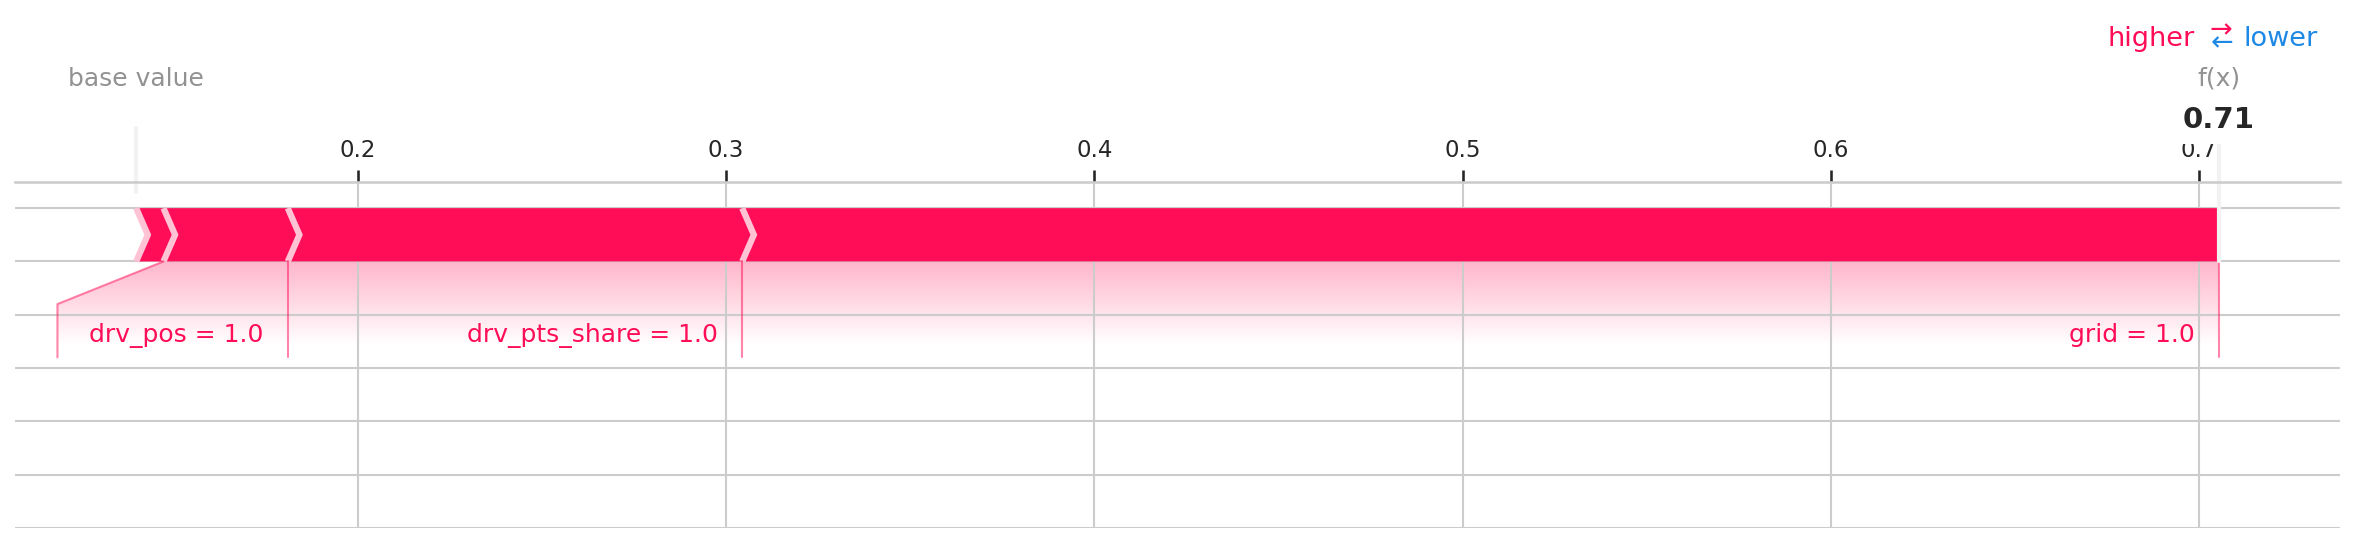
\includegraphics[width=0.85\linewidth]{fig_24_force_hit_lr.png}\\
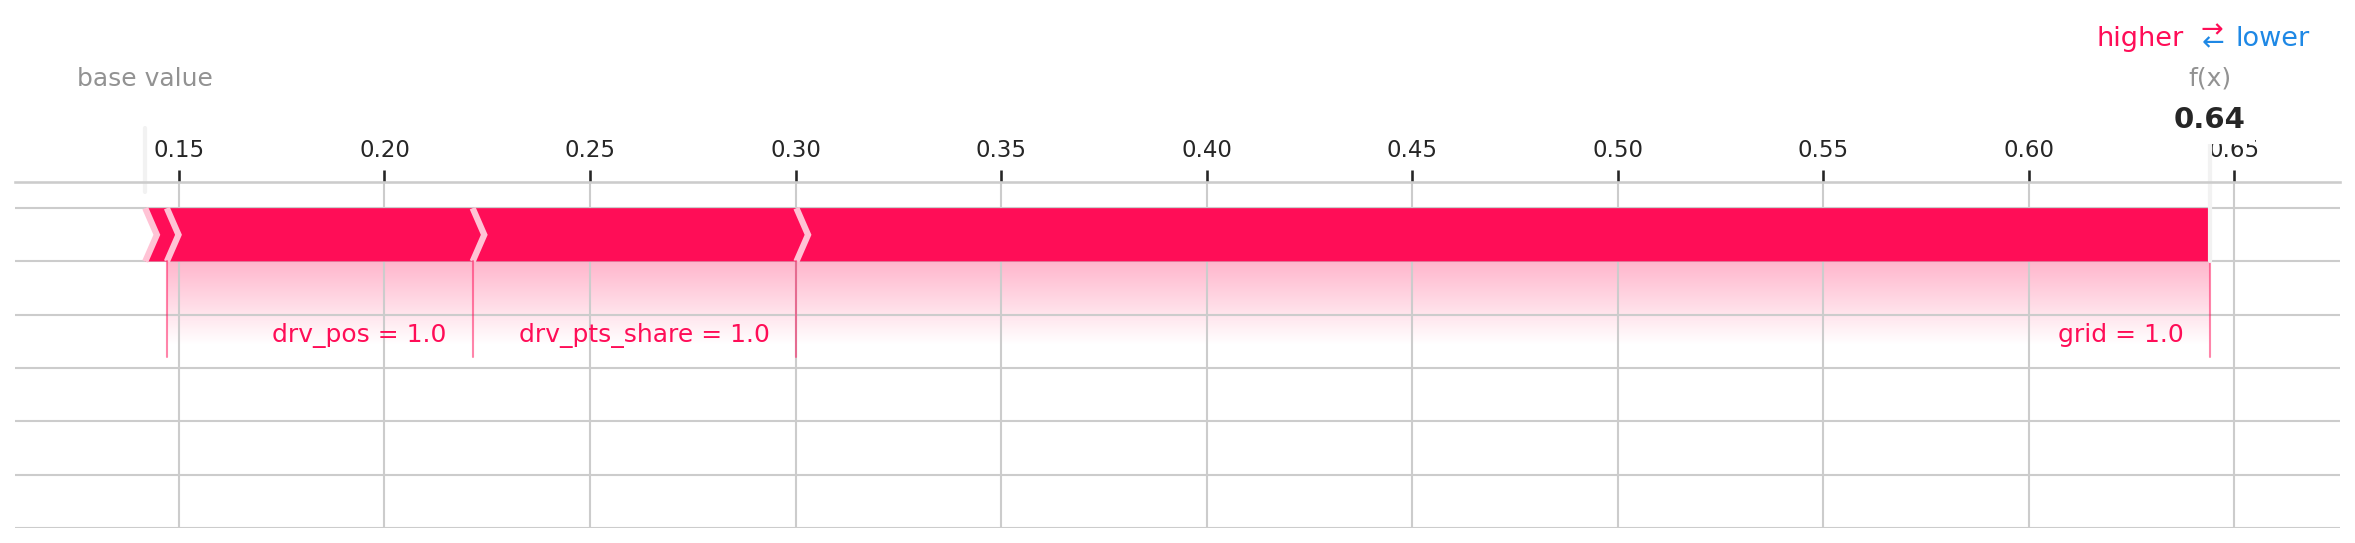
\includegraphics[width=0.85\linewidth]{fig_24_force_hit_rf.png}\\
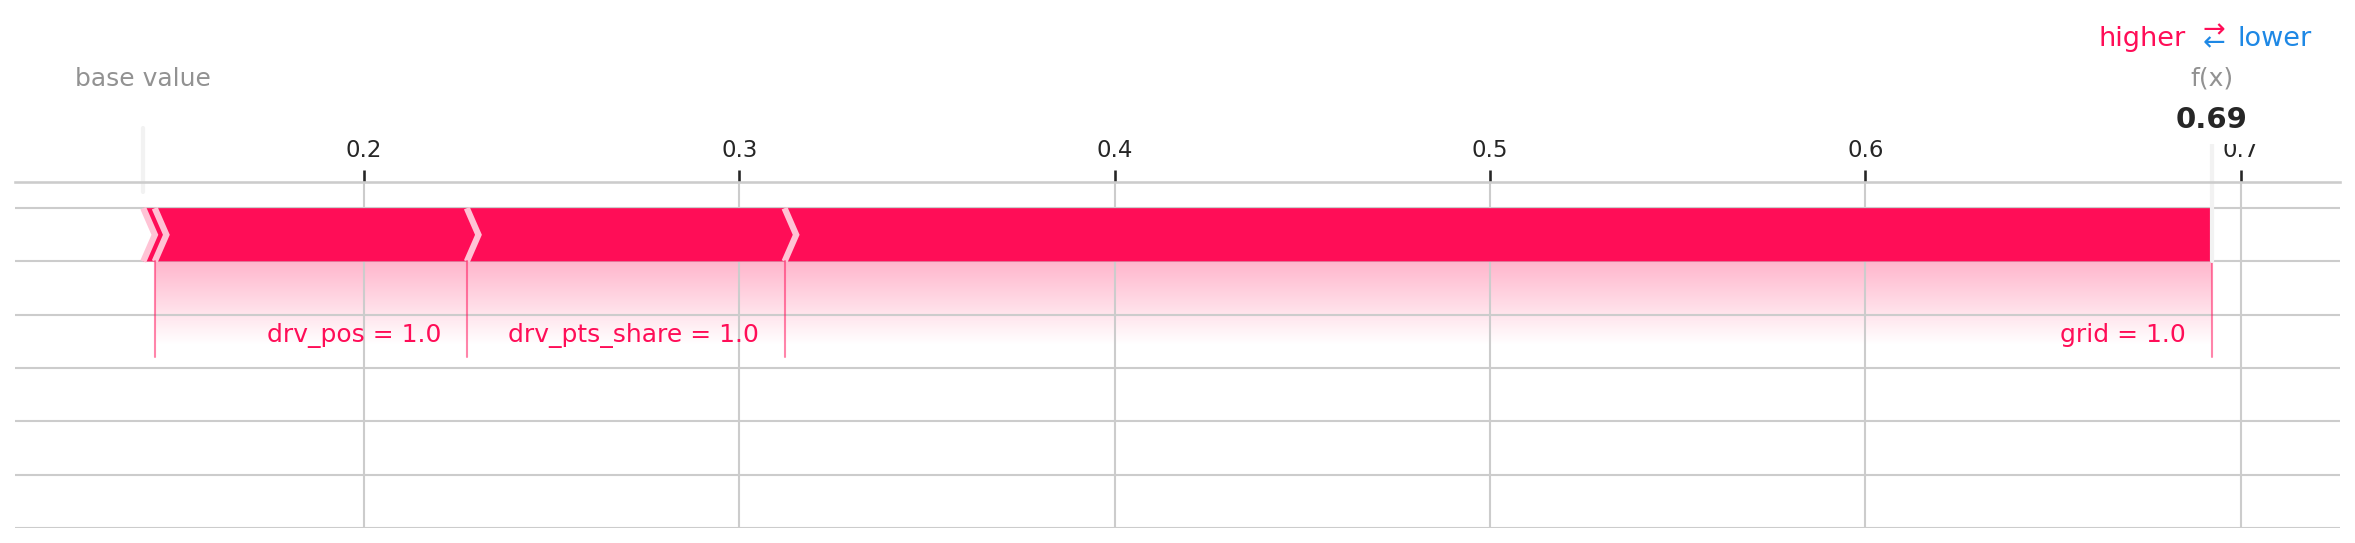
\includegraphics[width=0.85\linewidth]{fig_24_force_hit_nn.png}\\[4pt]
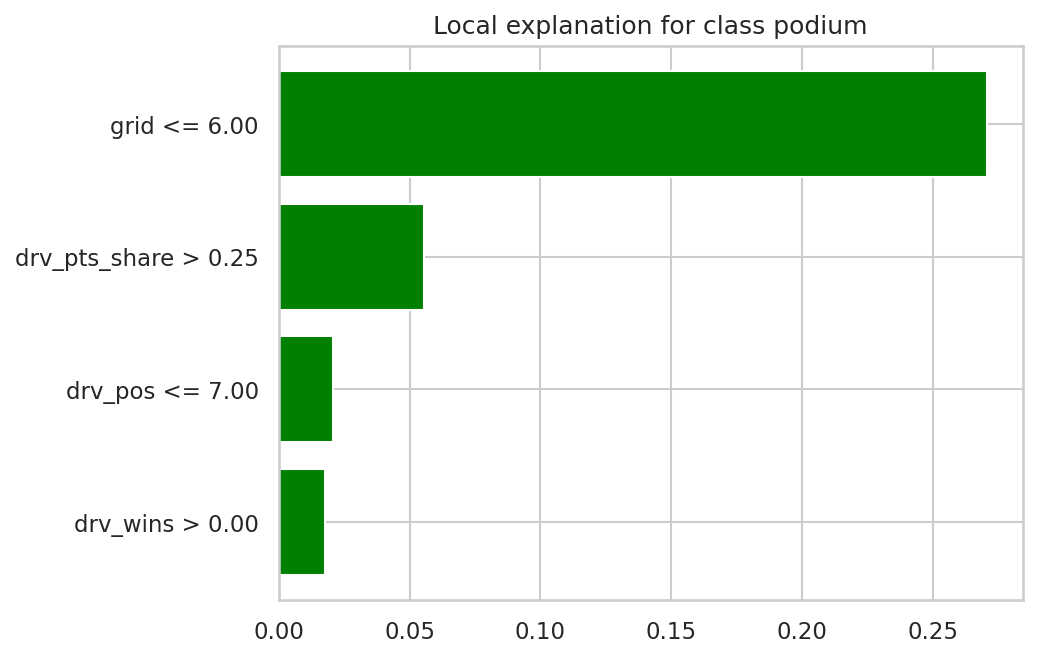
\includegraphics[width=0.32\linewidth]{fig_25_lime_hit_lr.png}\hfill
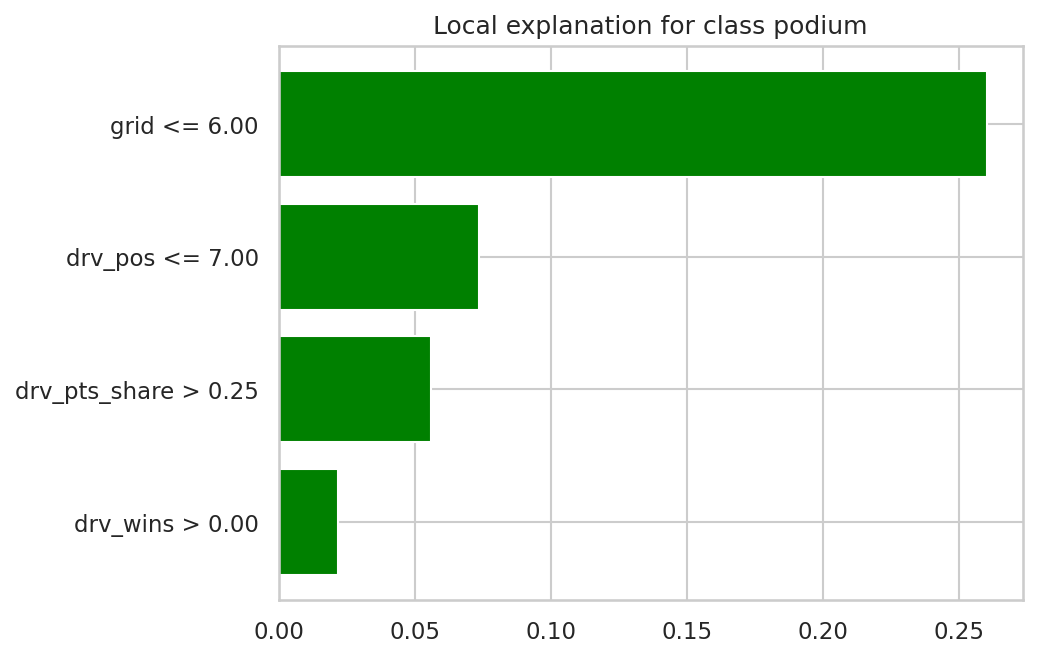
\includegraphics[width=0.32\linewidth]{fig_25_lime_hit_rf.png}\hfill
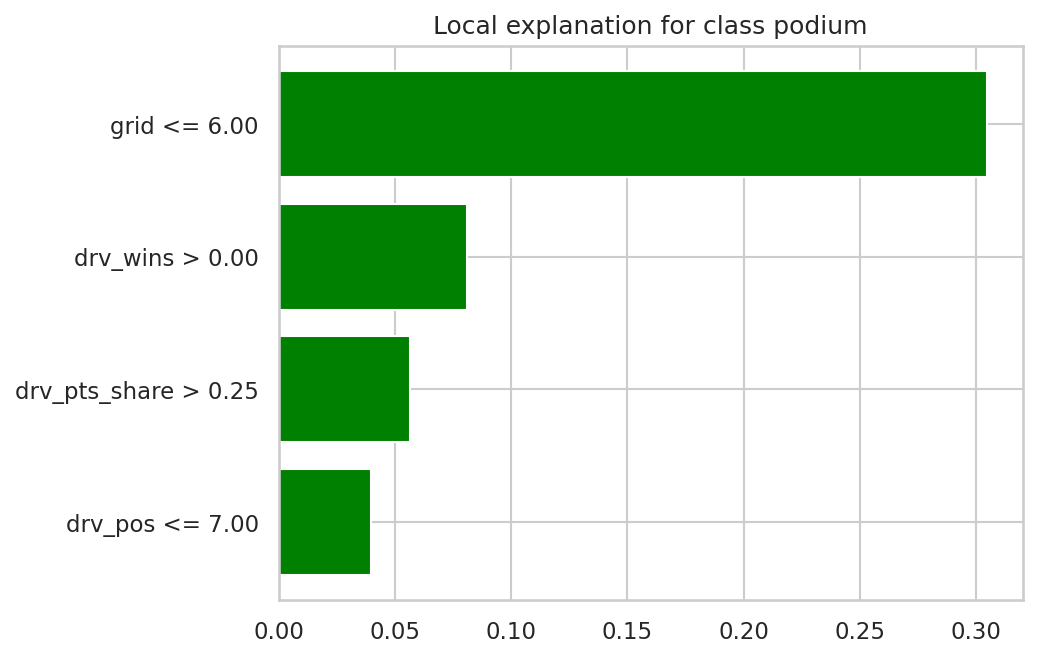
\includegraphics[width=0.32\linewidth]{fig_25_lime_hit_nn.png}
\caption{Hit: Sebastian Vettel, 2018 Bahrain GP. Top: SHAP force plots for logistic regression, forest and network (red pushes up, blue down, from the base value to $f(x)$). Bottom: LIME for the same three (green = towards podium, red = against).}
\label{fig:localhit}
\end{figure}

\begin{figure}[H]
\centering
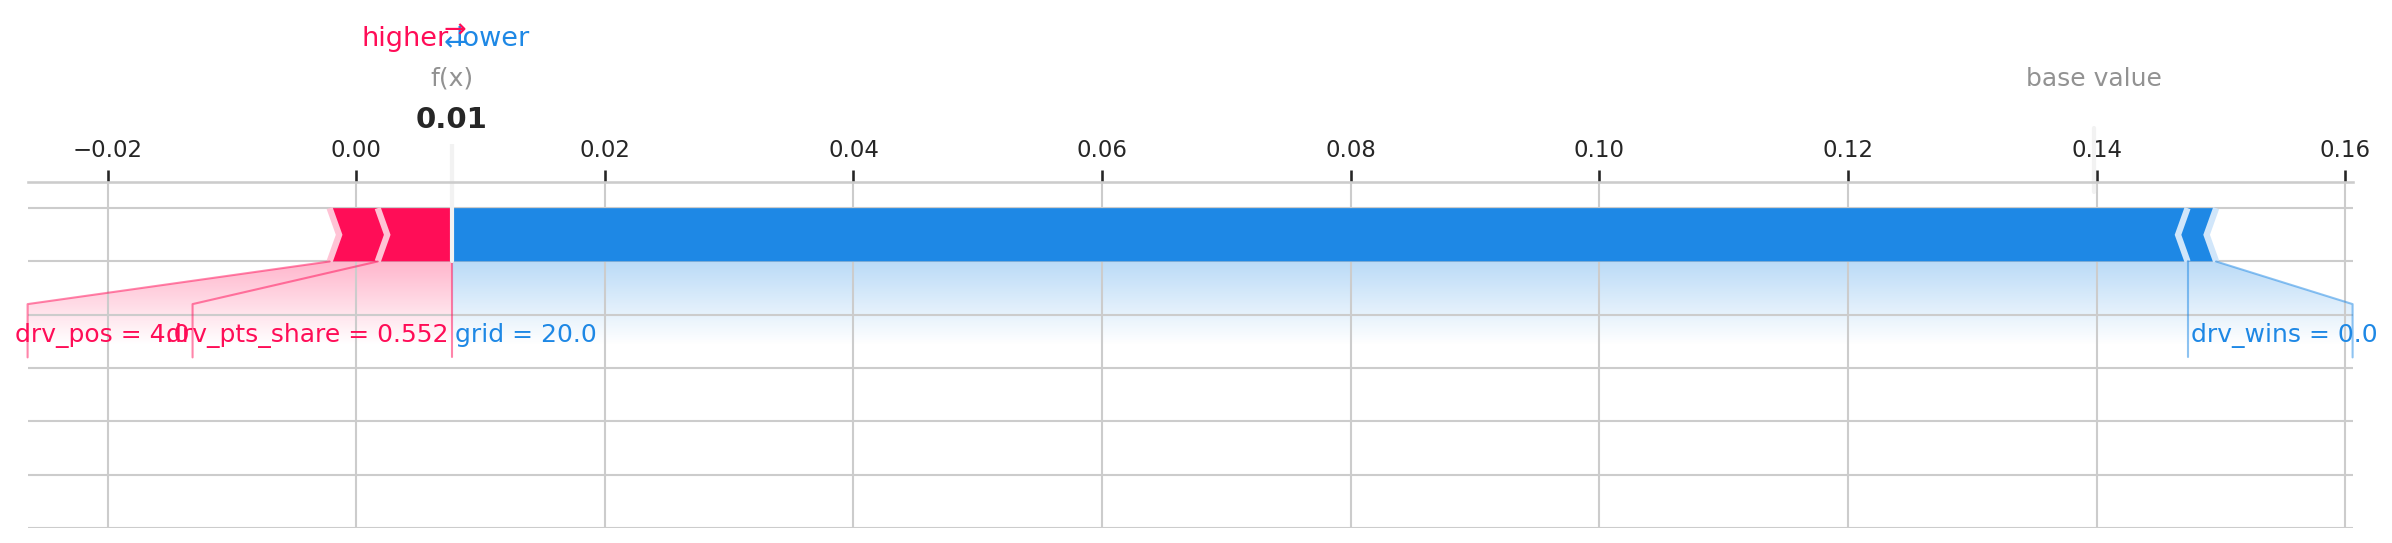
\includegraphics[width=0.85\linewidth]{fig_24_force_miss_lr.png}\\
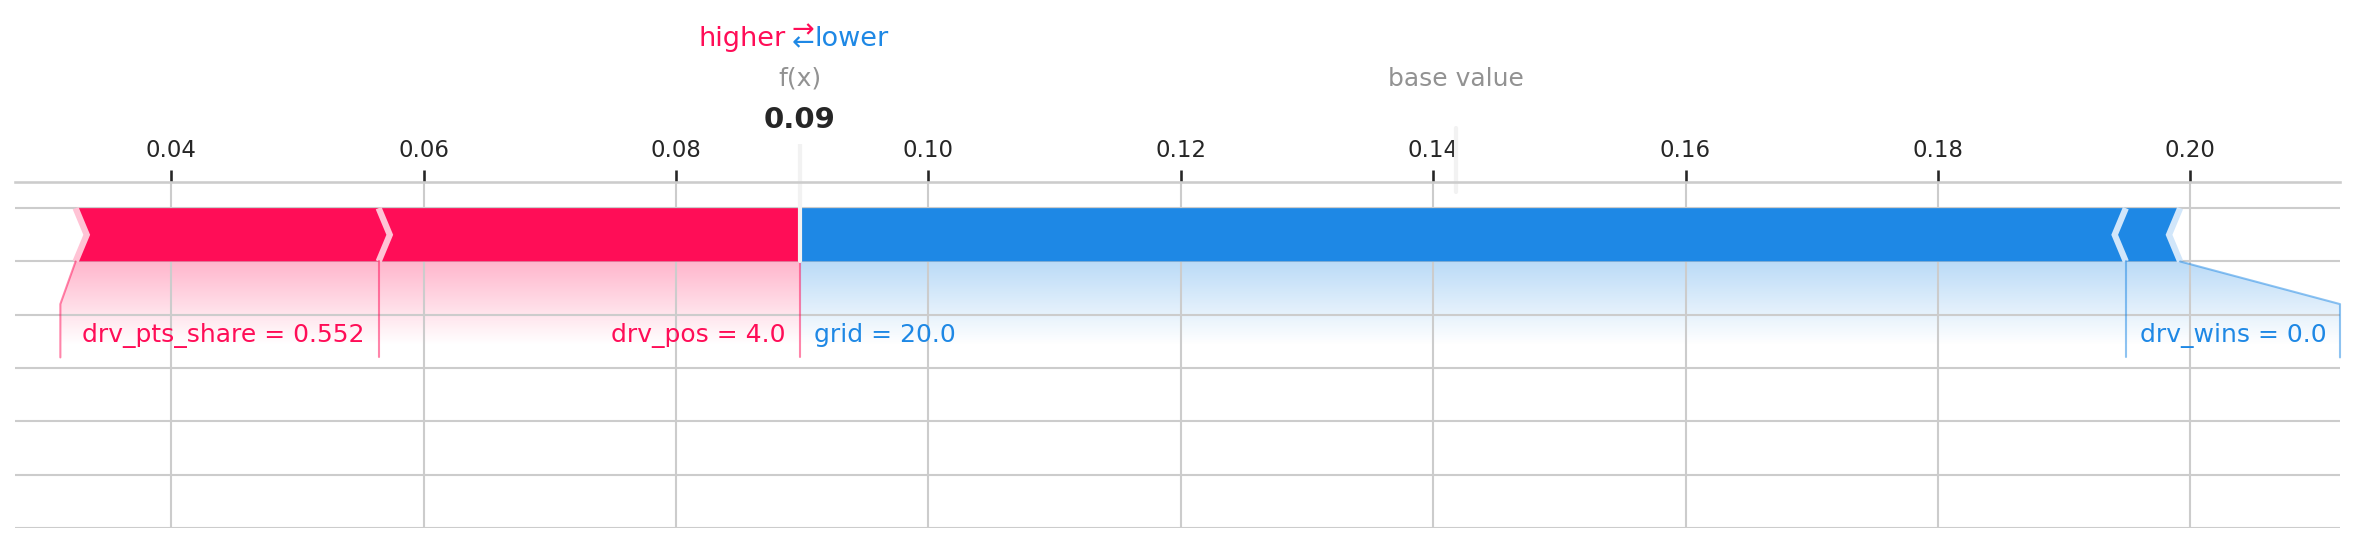
\includegraphics[width=0.85\linewidth]{fig_24_force_miss_rf.png}\\
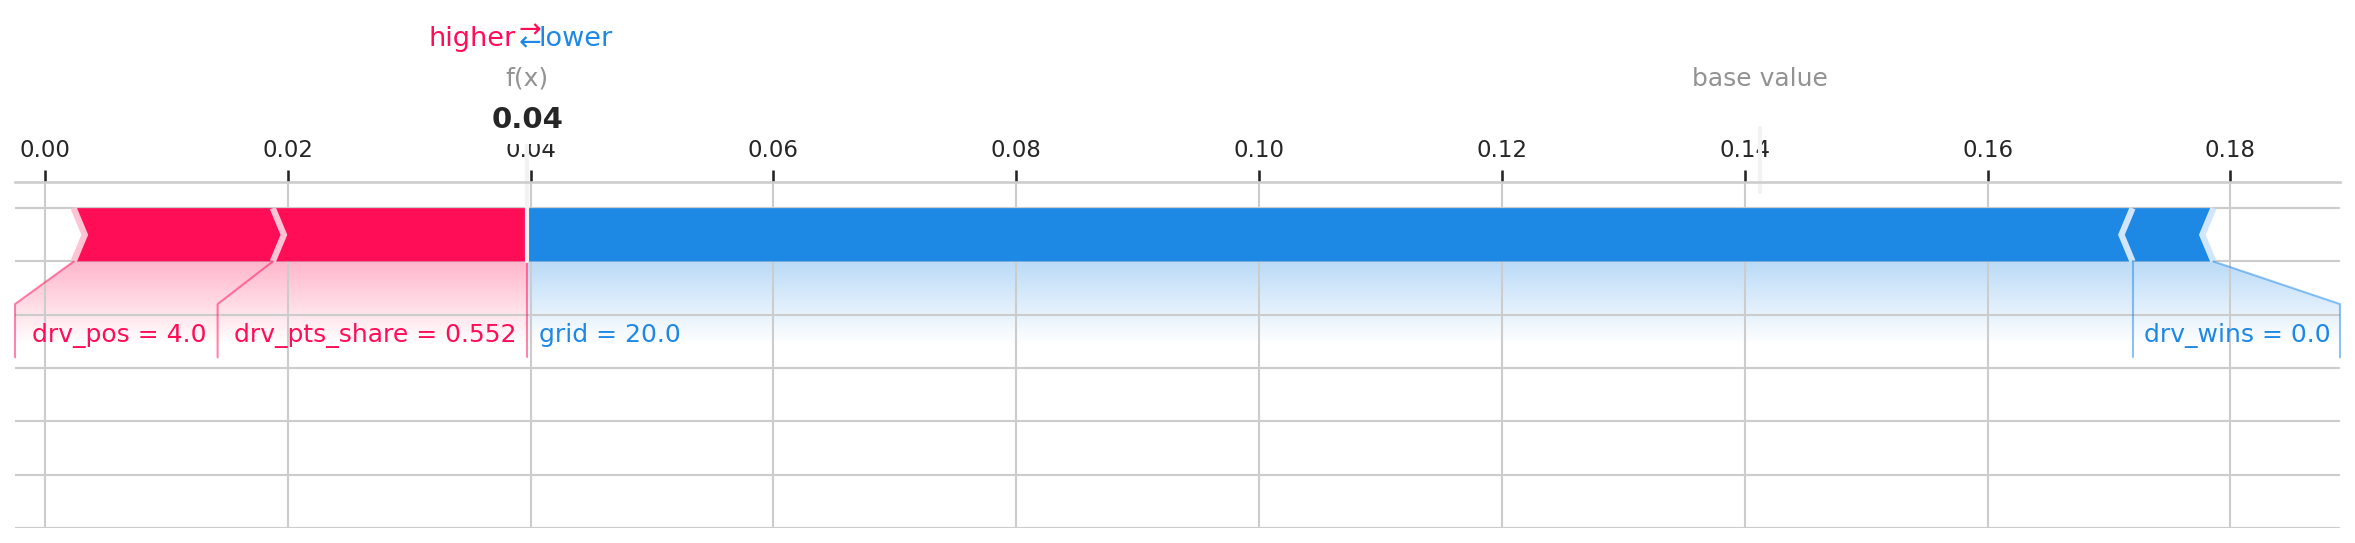
\includegraphics[width=0.85\linewidth]{fig_24_force_miss_nn.png}\\[4pt]
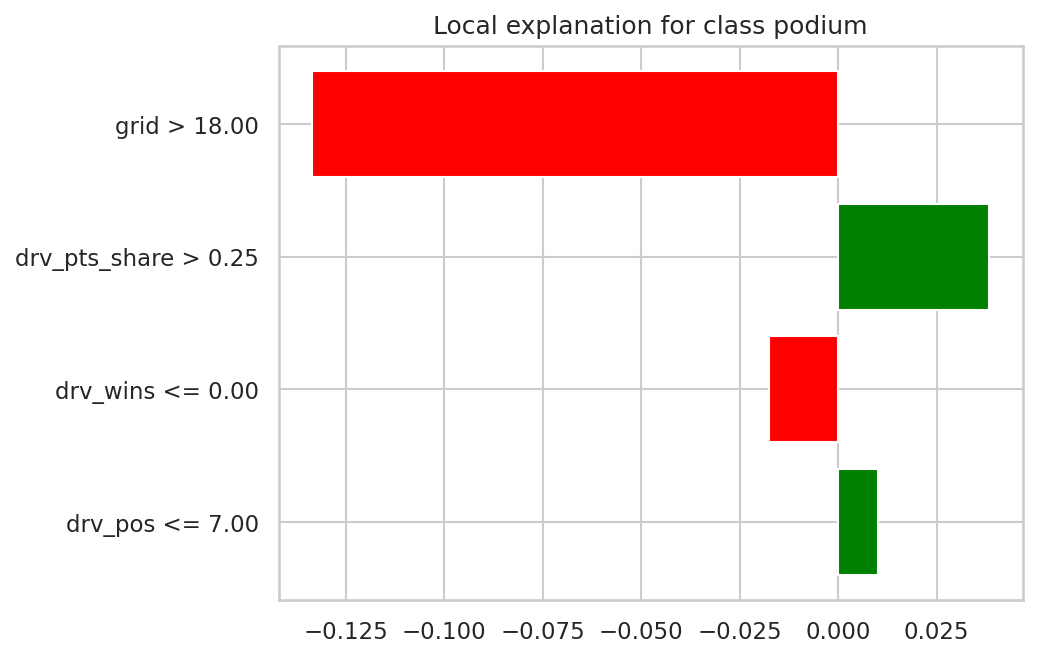
\includegraphics[width=0.32\linewidth]{fig_25_lime_miss_lr.png}\hfill
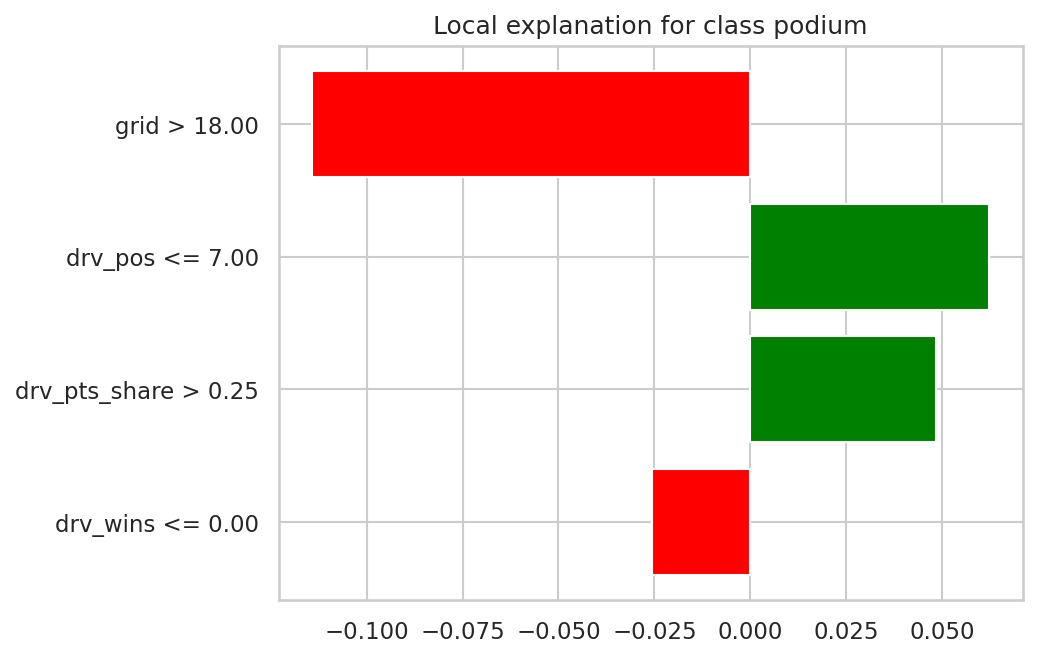
\includegraphics[width=0.32\linewidth]{fig_25_lime_miss_rf.png}\hfill
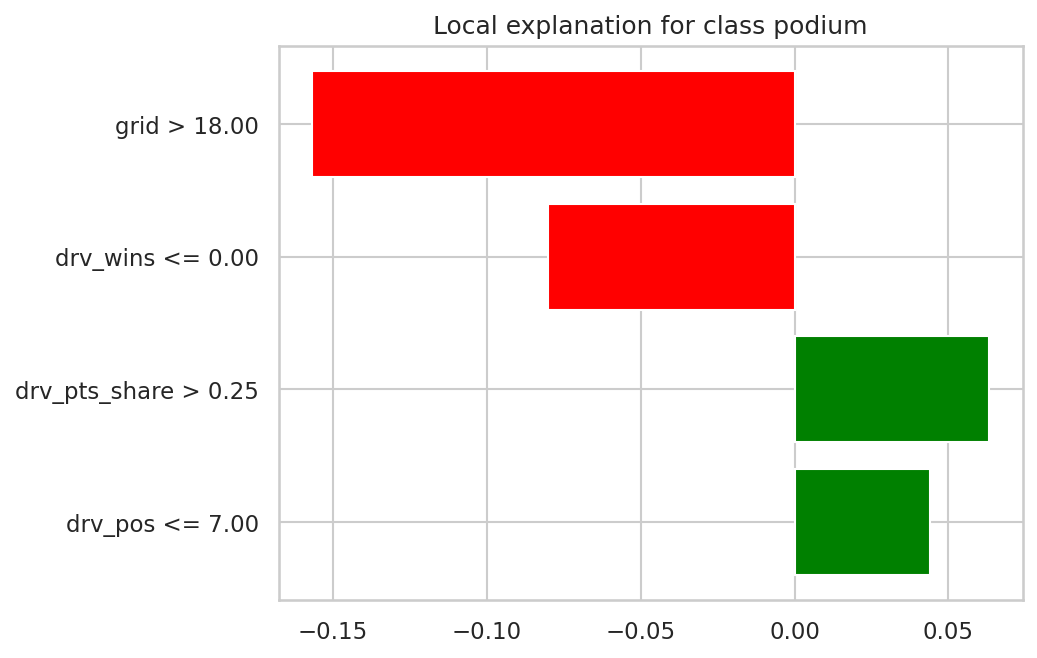
\includegraphics[width=0.32\linewidth]{fig_25_lime_miss_nn.png}
\caption{Miss: Sebastian Vettel, 2019 German GP. Same layout as \fig{fig:localhit}.}
\label{fig:localmiss}
\end{figure}

\begin{table}[H]
\centering\small
\caption{SHAP values and LIME weights for the forest, and each model's probability.}
\label{tab:local}
\begin{tabular}{lrrrcrrr}
\toprule
 & \multicolumn{3}{c}{Hit: Vettel, Bahrain 2018} && \multicolumn{3}{c}{Miss: Vettel, Germany 2019} \\
\cmidrule{2-4}\cmidrule{6-8}
Input & Value & SHAP & LIME && Value & SHAP & LIME \\
\midrule
\code{grid} & 1 & $+0.344$ & $+0.260$ && 20 & $-0.105$ & $-0.114$ \\
\code{drv\_pos} & 1 & $+0.074$ & $+0.074$ && 4 & $+0.033$ & $+0.062$ \\
\code{drv\_pts\_share} & 1.00 & $+0.079$ & $+0.056$ && 0.552 & $+0.024$ & $+0.048$ \\
\code{drv\_wins} & 1 & $+0.005$ & $+0.022$ && 0 & $-0.004$ & $-0.026$ \\
\midrule
$P(\text{podium})$ LR / RF / NN & \multicolumn{3}{c}{0.71 / 0.64 / 0.69} && \multicolumn{3}{c}{0.01 / 0.09 / 0.04} \\
LIME local fit $R^2$ (3 models) & \multicolumn{3}{c}{0.80--0.83} && \multicolumn{3}{c}{0.22--0.27} \\
\bottomrule
\end{tabular}
\end{table}

\textbf{Reading.} \emph{Hit:} the championship leader on pole; every model says podium, above its threshold. For the forest, from the average of about 0.14, \code{grid = 1} adds the most, then the points share and the position; one win adds almost nothing. The other models also put the grid first.
\emph{Miss:} Vettel started 20th and finished on the podium; every model says no. \code{grid = 20} pulls the probability down ($-0.11$ to $-0.14$ across the models), while the driver's standings (4th, 55\% of the leader's points) push it up a little. Given what is known before the start a low probability is right: only 1.6\% of starts from 11th or further back end on the podium (Q2). The race was wet (outside knowledge), which nothing before the start can show.
SHAP and LIME point the same way for every input, row and model. LIME's local fit is good for the hit and poor for the miss, so for the miss the SHAP values are more trustworthy. SHAP splits the difference from the average exactly among the inputs; LIME's weights come from an approximate local model and need not add up.

%==============================================================================
\section{Inference functions}

\code{PREDICT[model]} is one inference function per model. Each takes one driver-race as a dictionary of pre-race features in their normal units, fills missing values with the training medians through the same imputer and scaler as in training, and returns the probability and the yes/no at that model's validation threshold. A key that is not a feature (a typo) is rejected instead of being treated as missing \nb{17}.

\begin{table}[H]
\centering\small
\caption{Inference on a complete record, a partially-missing record and a real test row with missing standings ($P(\text{podium})$, yes if above the model's threshold).}
\label{tab:inference}
\begin{tabularx}{\linewidth}{>{\raggedright\arraybackslash}Xrrrr}
\toprule
Record & Baseline & LR & RF & NN \\
\midrule
Complete: Verstappen, Saudi Arabian GP 2024 (grid 1, leader, 1 win); finished on the podium & 0.591 yes & 0.705 yes & 0.644 yes & 0.692 yes \\
Partially missing: only \code{grid = 4} (a rookie in round 1; standings filled with 12, 0.076, 0) & 0.348 no & 0.240 no & 0.338 no & 0.271 no \\
Real test row: Leclerc, Bahrain GP 2022 (round 1, standings missing); finished on the podium & 0.591 yes & 0.416 yes & 0.477 yes & 0.504 yes \\
\midrule
Thresholds & 0.427 & 0.399 & 0.432 & 0.348 \\
\bottomrule
\end{tabularx}
\end{table}

%==============================================================================
\section{Limitations}
\begin{itemize}
\item \textbf{Qualifying-coverage drift.} Qualifying times exist only from 1994 (Q2 from 2005, Q3 from 2006, and only for the faster drivers). The models use the grid and no qualifying times, so information such as the gap to pole is not used.
\item \textbf{Era sensitivity.} Field sizes, points systems and reliability changed a lot over 75 years. Points are a share of the leader's points and the split is by season, but the 1950s training rows still differ strongly from 2022--2024, and the test seasons are a new set of car rules.
\item \textbf{Dominant teams.} Mercedes took 45\% of validation podiums and Red Bull 37\% of test podiums, so the scores and explanations describe those eras.
\item \textbf{Race-day events are invisible.} Rain, crashes, safety cars and failures are not known before the start; the miss row is an example.
\item \textbf{Small validation and test sets} (243 and 204 podiums): differences of about 0.01 PR-AUC between models could turn around with other seasons.
\item \textbf{One validation block does several jobs} (form window, feature groups, settings, early stopping, thresholds), so validation scores are a little optimistic.
\item \textbf{Missing standings are filled as a typical driver} (the training median); a round-1 favourite looks like a mid-table driver. No constructors' standings exist before 1958, and the 1950--1960 standings include Indy~500 drivers (33--44 per season), which pushes other drivers' positions down.
\item \textbf{Feature selection adds whole groups in a fixed order,} and only grid, field size, standings and form were candidates. Sprint results are not used.
\item \textbf{Q1--Q3} rely on our own grouping of 137 statuses and a nationality-to-country mapping; renamed teams are kept apart.
\item \textbf{Explanations are not causal} and describe these models on 2018--2021 rows.
\end{itemize}

%==============================================================================
\section{Conclusion}
After auditing and cleaning the 14 tables, a leakage-safe table of 24{,}933 entries was built and split by season.
Front-row starts convert to podiums far more often since 2014 (55.5\% $\rightarrow$ 76.0\%) and the circuit ranking reshuffled completely; there is no home advantage once the starting position is held fixed; and mechanical retirements fell from 11.2\% to 6.9\% of starts.
For prediction, the grid plus the driver's standings before the race are enough: logistic regression, a random forest and a shallow network all clearly beat the grid-only baseline (test PR-AUC 0.706--0.720 against 0.647) and are about equally good. Ablation and SHAP agree that the grid carries most of the signal and the season standings add a smaller but consistent part.

\bibliographystyle{plain}
\bibliography{references}

\appendix
\section{Reproducibility and methods}
The notebook runs top to bottom with \textit{Run All}. On Kaggle the CSV folder is found automatically and the first cell installs \code{shap}, \code{lime} and \code{missingno}; the versions used (Python 3.13, numpy 2.1.3, pandas 2.3.3, scikit-learn 1.6.1, TensorFlow 2.20.0, shap 0.52.0, lime 0.2.0.1) are printed by the second cell and pinned in \code{environment.txt}. All random seeds are 42.

\begin{table}[H]
\centering\small
\caption{Methods used and where they come from.}
\label{tab:methods}
\begin{tabularx}{\linewidth}{>{\raggedright\arraybackslash}p{5.4cm}>{\raggedright\arraybackslash}Xl}
\toprule
Method & Question it answers & From \\
\midrule
\code{read\_csv}, \code{info}/\code{describe}, missingno & What is in the tables, what is missing & Lab 1 \\
Median imputation, \code{StandardScaler} fit on train & Fill gaps and scale without leaking & Labs 1, 3 \\
Logistic regression, random forest & Statistical models and baseline & Labs 2, 4 \\
Keras network, early stopping & Shallow neural network & Lab 3 \\
PR-AUC, ROC-AUC, F1, precision, recall & Prediction quality & Lab 2, brief \\
SHAP (permutation, \code{TreeExplainer}), LIME & Global and local explanations & Lab 4, brief \\
Wilson interval & Uncertainty of a rate from few cases & Wilson (1927) \\
Spearman correlation & Monotonic relations, rankings & rank version of Lab 1 \\
Odds ratio from logistic regression & Home effect at the same start and era & Lab 2 model \\
VIF & Is a column mostly a copy of the others & Lab 2 linear regression \\
Race bootstrap & Can two windows / two feature sets be told apart & Efron \& Tibshirani (1993) \\
\bottomrule
\end{tabularx}
\end{table}

\end{document}
